\chapter{面向策略整合的偏序协同对抗学习方法}

\section{问题的提出}


\subsection{金融市场非对称博弈结构与层级关系}

本章进入对冲基金交易决策流程的最后环节，讨论最终交易判断与策略整合问题。第2章关注资产选择与资金配置，第3章讨论资产选择背后的因子依据，第4章判断趋势结构与交易时机，第5章处理信号进入市场后的执行路径。上述环节分别解决了交易链条中的局部问题，但真实交易系统还需要把这些判断转换为买入、卖出或持有动作。基于此，本章提出面向策略整合的偏序协同对抗学习方法，将涨、跌、平分类结果解释为最终交易判断的输出形式，而不是孤立的价格方向预测。

从交易机制看，策略整合并不是简单汇总若干预测信号，而是需要在市场状态、参与者结构、资产配置结果和执行约束之间建立层级化决策关系。金融市场中的主体并不处于完全对称的位置：机构资金、高频做市商、套利资金与普通投资者在信息获取速度、资金体量、持仓约束和执行能力上均存在差异。价格方向的形成，往往是这些异质主体在不同时间尺度上反复博弈后的结果。因此，本章讨论的涨、跌、平分类结果，本质上是策略整合后的买入、卖出或持有判断，而不是静态样本上的普通分类标签。

早期统计模型和浅层机器学习方法为金融预测提供了基础工具，但它们通常更依赖预设变量、固定窗口或人工构造特征。随着深度学习方法进入金融预测领域，研究者开始利用多层非线性结构从价格序列中学习更复杂的表征。不过，这类方法主要解决价格序列表征和方向预测问题，即使能够提高局部拟合能力，也并不自动解决多源信息如何进入最终交易决策的问题。对本章而言，方向预测只能构成策略整合的前置环节，真正需要回答的是预测信号如何与资产配置、因子依据、结构判断和执行约束共同形成买入、卖出或持有决策。

对策略整合而言，最直接的困难来自金融市场的非平稳性。自适应市场假说强调，市场有效性会随参与者行为和环境变化而动态演化\cite{lo2004adaptive}。计量经济学中的状态切换模型也说明，金融序列可能在不同机制之间转换，而不是始终服从单一稳定分布\cite{hamilton1989regime}。这意味着模型在某一阶段学到的分类边界，可能会在后续市场环境中失效；尤其当趋势行情转入震荡，或低波动环境突然切换为高波动环境时，原有判别规则容易出现系统性偏移。若这种偏移直接进入最终策略输出，就可能导致买入、卖出或持有判断失真。

更进一步，方向预测的价值并不只取决于分类准确率。金融预测研究早已指出，统计预测能力与交易经济价值之间可能存在明显差异\cite{leitch1991economic}。在实际交易中，预测信号还需要进入仓位调整、资产配置和执行环节。因此，本章关注的不是单纯提高某个分类器的离线准确率，而是讨论方向分类结果如何在策略层面转化为最终交易判断。这里的“承接”并不意味着直接调用前述各章实验输出，而是指第6章在问题定义、模型解释和评价口径上延续前序交易环节，使涨、跌、平输出能够对应买入、卖出或持有动作。

基于上述背景，本章将偏序协同对抗（Partial-order Collaborative Adversarial, PCA）引入策略整合任务。其定位不是重新提出与第2章并列的基础架构，而是在前文分别讨论资产配置、因子依据、结构识别与执行约束之后，进一步组织层级博弈关系、分类边界校正、异常修复约束和交易方向输出。该方法通过生成器与多组判别器之间的非对称配置刻画不同市场主体之间的层级差异，并按群组交叉对抗、赛马场竞争、逆向师生蒸馏和孪生对抗自体再生的顺序约束训练过程，从而降低分类边界漂移、样本噪声扰动和局部模式崩溃对最终交易判断的影响。


\subsection{涨跌分类中的模式崩溃与稳健性挑战}

在策略整合环节，涨跌分类承担的是最终交易动作映射功能，即将多源信息压缩为买入、卖出或持有判断。其难点不只在于提高分类准确率，更在于分类结果是否能够稳定承接资产配置、因子解释、时序结构和执行约束。如果分类边界在非平稳市场中发生漂移，最终交易决策就可能出现方向反转、过度交易或信号失效。

从已有金融机器学习研究看，非线性模型确实能够从大规模资产特征中提取传统线性模型难以表达的信息，并在部分预测任务上表现出优势\cite{gu2020empirical}。但这类优势通常依赖样本结构、特征处理和评价方式。一旦市场状态发生变化，单一模型往往会出现两个问题：一是对历史噪声过度拟合，二是对未来样本中的新模式反应迟缓。对于策略整合而言，这两个问题都会直接表现为最终交易动作的不稳定，例如买入信号提前、卖出信号滞后或持有状态被错误打破。

对抗学习为缓解上述问题提供了一种可行路径。生成式对抗方法能够通过生成器与判别器之间的博弈学习数据分布，并已被用于金融数据生成、样本增强和分布建模等场景\cite{cui20241gan}。然而，对抗训练自身也存在模式崩溃风险：生成器可能只覆盖少数“安全”模式，判别器则可能对这些局部模式形成过强偏好。模式崩溃问题在一般生成对抗网络中已经较为突出，在高噪声、厚尾和状态切换频繁的金融数据中会更加明显\cite{barsha2024review}。当这种崩溃发生在策略整合阶段时，其影响不再局限于分类误差，而会进一步传导到仓位方向、交易频率和风险暴露。

因此，本章的稳健性目标并不是简单增加模型数量，而是让不同模型在有序约束下形成互补。单纯的平均集成或投票集成只能在输出层合并结果，无法保证内部表征真正多样；而偏序协同对抗要求生成器、判别器组、学生模型和孪生修复机制按固定顺序发挥作用，使系统在出现局部失效时能够通过后续机制进行校正。换言之，本章试图解决的不是“再训练一个更强分类器”，而是如何让分类信号在策略整合阶段稳定承接资产、因子、结构和执行四类决策信息，并转化为可解释、可恢复、可执行的最终交易决策。

据此，本章需要回答三个关键问题：其一，如何将多源交易信息纳入有序的最终判断过程，避免涨跌分类与前序交易环节脱节；其二，如何在非平稳市场和层级博弈结构下抑制分类边界漂移与模式崩溃；其三，如何使涨、跌、平输出真正对应买入、卖出或持有动作，而不是停留在离线分类指标层面。PCA的设计正是围绕这三个问题展开。


\section{相关工作}

围绕策略整合与最终交易决策，已有研究主要集中在三个方向：一是基于高频限价指令簿和市场微观结构的方向预测研究，二是基于深度学习与对抗学习的金融分类方法，三是将预测信号转化为交易动作和策略表现的决策映射研究。限价指令簿数据在中间价预测与高频方向分类中被广泛使用，其难点在于同时刻画盘口局部结构、时间依赖与交易方向之间的关系\cite{ntakaris2018benchmark}。在本文整体逻辑中，这类方向信号不是孤立的分类结果，而是承接前文投资组合管理、高维金融因子建模、时序结构识别和交易执行优化后的策略整合输入。

在金融方向预测研究中，深度序列模型被用于从历史价格序列中提取非线性时序依赖。长短期记忆网络在股票方向预测中的实证研究表明，序列模型能够在部分样本上取得优于传统方法的表现\cite{fischer2018deep}。这类研究说明，金融时间序列中的长期依赖关系可以通过深层模型得到更充分的刻画。
在此基础上，注意力机制进一步被用于突出关键时间片段，使模型能够在价格变化过程中识别更重要的局部信息\cite{chen2019attlstm}。这一路径的意义在于，它不再仅依赖整体序列拟合，而是试图解释哪些阶段的信息对方向判断更为关键。

除直接建模价格序列外，也有研究将分解算法与深度学习结合，以提升复杂价格序列中的结构提取能力\cite{zhang2021based}。这些研究说明，深度学习方法能够改善方向预测中的特征表达，但其重点仍主要落在预测精度或局部表征能力上。对于本章讨论的策略整合任务而言，更关键的问题是：这些预测信号如何进一步进入最终交易动作，而不是停留在离线分类结果层面。
除直接处理原始价格序列外，也有研究将技术指标转化为图像形式，并利用二维卷积神经网络进行交易信号分类\cite{sezer2018algorithmic}。这类方法说明，金融分类任务中的特征组织方式会影响方向识别效果，但其重点仍在输入表征与离线分类表现上。
也有研究从层次化消息传递角度刻画金融方向预测问题，强调不同市场信息层级之间的交互关系\cite{ding2020hmsg}。这类研究与本文关注的层级组织思想具有一定关联，但其重点仍主要是方向预测模型本身。
动态多尺度注意力模型进一步从不同时间尺度捕捉价格运动特征，为金融方向预测提供了多尺度建模思路\cite{yoo2021dtml}。不过，已有研究通常仍以预测性能为中心，对预测结果如何进入最终买入、卖出或持有判断讨论不足。

与普通监督分类相比，策略整合环节的涨、跌、平输出不仅要对应标签预测，还要能够映射到买入、卖出或持有判断。已有分类研究通常更关注离线准确率或单一数据结构下的预测表现，而真实交易系统还需要处理状态切换、边界模糊和信号冲突等问题。因此，分类模型能否在非平稳市场中保持稳定边界，并将预测结果转化为可执行的策略输出，是本章进一步讨论的重点。
在交易决策映射方面，动态资产配置可以被视为连续状态下的序列决策过程，相关深度强化学习投资组合研究已从仓位调整和资产配置角度提供了参考\cite{xiao2025research}。不过，本章关注的不是单一组合权重更新，而是把涨跌分类放入买入、卖出或持有的最终判断流程中，使分类输出能够与前序资产、因子、结构和执行信息形成衔接。
对抗学习和多模型协同为上述问题提供了可借鉴思路，但若多个机制并列作用，训练过程容易出现目标冲突或震荡。本章采用偏序协同方式组织GCA、赛马场竞争机制、逆向师生蒸馏机制与孪生对抗自体再生机制，使其按照基础对抗、动态筛选、知识校正和异常修复的顺序进入策略整合流程，从而避免将多源机制简单叠加。

已有研究分别在方向预测、金融分类、对抗学习和交易决策映射等方面形成积累，但分类边界稳定性、机制修复能力和最终交易动作之间仍缺少清晰衔接。本章在此基础上，把涨跌分类放回对冲基金交易决策链条的最后环节中讨论。


\section{偏序协同对抗方法}

本节在相关工作基础上介绍PCA的模型结构、损失函数与训练流程。这里的偏序协同对抗方法服务于策略整合任务，即将方向分类、模型置信度和异常修复状态共同转化为买入、卖出或持有判断。与第2章侧重多资产资金配置、第3章侧重因子依据筛选、第4章侧重时序结构识别、第5章侧重执行路径优化不同，本章方法的落脚点是最终交易判断，因此模型结构中的生成、判别、筛选、蒸馏和修复环节都围绕“方向输出能否稳定形成交易动作”展开。令 $X_t = [x_{t-T+1}, \dots, x_t] \in \mathbb{R}^{T \times F}$ 表示截止时刻 $t$ 的历史时间步序列，其中 $T$ 为时间窗口长度（本章设定为120），$F$ 为特征维度。

偏序协同对抗架构采用非对称的多组多成员结构，目标是在同一训练流程中同时约束序列生成、趋势判别与买卖持有映射。
生成器负责捕捉市场微观结构并生成未来开盘价、最高价、最低价、收盘价与成交量序列。本文采用基于自注意力机制的序列到序列生成器，输入长度为120的历史窗口，通过4头自注意力、2层编码器和维度为512的前馈网络提取时序特征，再以自回归方式生成未来序列，随机失活率设为0.1。
判别器在PCA架构中扮演着双重角色：既是区分真实与生成数据的“裁判”，也是预测未来趋势的“分析师”。为此，我们设计了支持卷积神经网络和自注意力序列模型两种架构的时序分类网络。

\begin{figure}[htbp]
\centering
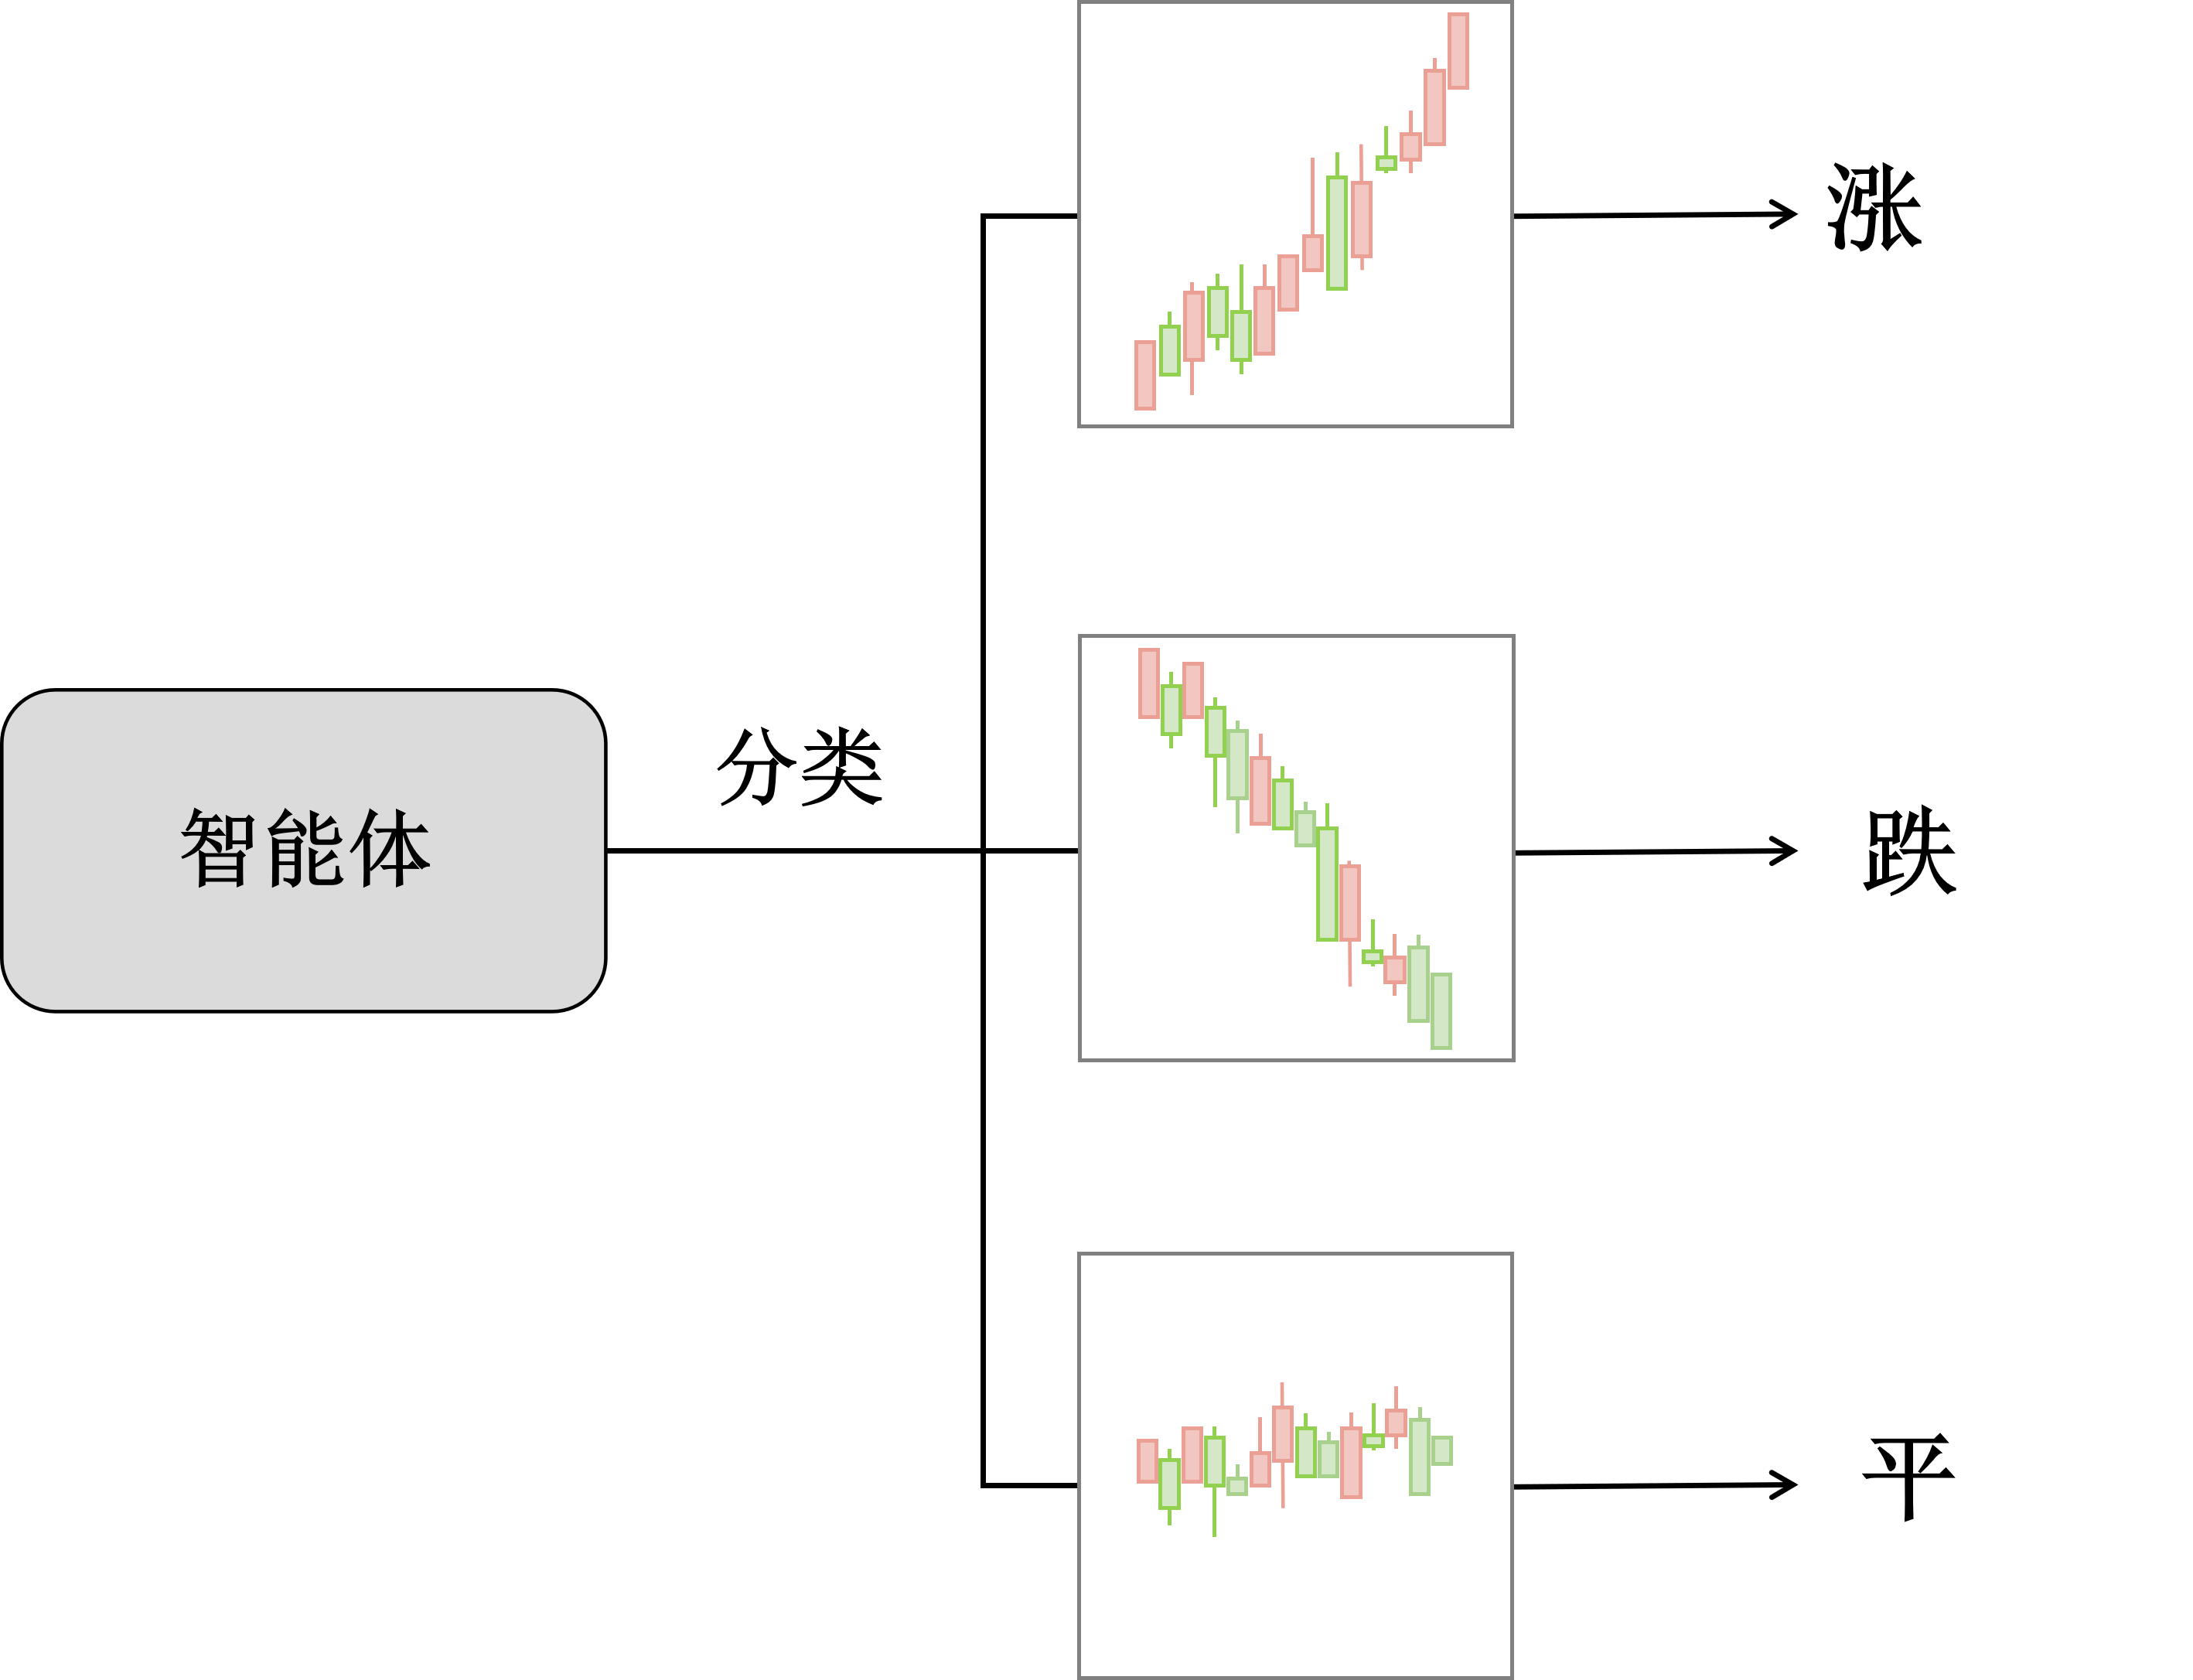
\includegraphics[width=0.5\textwidth]{figures/chap7/偏序/分类任务.png}
\caption{策略整合中的方向输出任务图}
\label{fig:twinclasstaskfig}
\end{figure}

如图\ref{fig:twinclasstaskfig}所示，不同于传统生成对抗网络判别器仅输出单一的真假标量，我们的判别器输出层包含两个关键分支：分类头输出一个3维的逻辑输出向量，对应未来价格的“涨、跌、平”三种趋势的概率分布，这使得判别器输出能够对应最终交易决策中的买入、卖出或持有判断；特征头直接输出倒数第二层的高维特征向量，为GCA和逆向师生蒸馏机制阶段的特征级蒸馏提供了必要的载体，使得落后模型能够直接学习最优模型的内部表征。
架构的关键在于“1个生成器组 × 1个成员、2个判别器组 × 每组3个成员”的非对称配置。预训练后的单个自注意力序列模型生成器持续提供虚拟样本；两个判别器组中的6个异构判别器交替采用卷积神经网络与自注意力序列模型结构。
在损失函数设计上，本文采用兼顾生成质量、分类精度与知识迁移的复合损失体系。

\textbf{（1）生成器金融感知重构损失。}生成器的核心损失函数为金融感知重构损失，该损失对开盘价、最高价、最低价与收盘价价格维度与成交量维度采用不同的损失函数，以适应金融数据的异质性特征。价格维度采用Huber损失，其在误差较小时等价于均方误差以保证平滑梯度，在误差较大时退化为线性损失以抑制价格跳变带来的梯度爆炸；成交量维度采用对数双曲余弦损失，其对零值和异常值具有天然的鲁棒性。两者通过权重系数加权求和：

\begin{equation}
\mathcal{L}_{G}^{\text{recon}} = w_p \cdot \text{Huber}_{\delta=1.0}(\hat{P}_{\text{开高低收}}, P_{\text{开高低收}}) + w_v \cdot \text{对数双曲余弦}(\hat{V}, V)
\label{eq:financial_aware_loss}
\end{equation}
其中$w_p=1.0$，$w_v=0.8$。
\begin{equation}
\text{Huber}_\delta(e) = \begin{cases} \frac{1}{2}e^2, & |e| \leq \delta \\ \delta\left(|e| - \frac{1}{2}\delta\right), & |e| > \delta \end{cases}
\end{equation}
\begin{equation}
\text{对数双曲余弦}(\hat{V}, V) = \frac{1}{N}\sum_{i=1}^{N}\log\left(\cosh(\hat{V}_i - V_i)\right)
\end{equation}

该设计突出价格信息的重要性，同时兼顾成交量这一辅助变量。

\textbf{（2）判别器分类损失。}判别器的损失函数采用基于三分类标签（涨/跌/平）的交叉熵损失：

\begin{equation}
\mathcal{L}_{D}^{\text{交叉熵}} = -\frac{1}{N}\sum_{i=1}^{N}\sum_{c=1}^{3} y_{i,c} \log(\hat{y}_{i,c})
\label{eq:disc_ce_loss}
\end{equation}

其中$c \in \{\text{涨}, \text{跌}, \text{平}\}$。相较于传统生成对抗网络中的二分类真假判别，这种设计迫使判别器不仅要区分数据的来源，更要将价格趋势逻辑转化为策略整合阶段的方向输出。

\textbf{（3）知识蒸馏损失。}在GCA组内对抗、组间对抗以及逆向师生蒸馏环节中，落后判别器通过最小化与最优判别器在特征层和输出层的均方误差实现知识迁移。知识蒸馏最初用于教师模型向学生模型传递软标签信息\cite{hinton2015distilling}。与单向蒸馏不同，深度互学习研究表明，多模型之间可以通过双向学习提升整体表示质量\cite{zhang2018deep}。后续蒸馏综述也表明，蒸馏机制不仅可用于模型压缩，也可用于表示对齐与训练稳定化\cite{huang2022distillation}：

\begin{equation}
\mathcal{L}_{\text{Distill}} = \lambda \cdot \left[\text{均方误差}(\mathbf{f}_i, \mathbf{f}^*) + \text{均方误差}(\mathbf{z}_i, \mathbf{z}^*)\right]
\label{eq:distill_loss}
\end{equation}

其中$\mathbf{f}_i$和$\mathbf{f}^*$分别为当前判别器和最优判别器倒数第二层的特征表示，$\mathbf{z}_i$和$\mathbf{z}^*$为对应的输出层逻辑输出，蒸馏权重系数$\lambda=0.1$。这一设计在保持判别器多样性的同时引导其向最优解收敛。与静态平均集成不同，蒸馏项在训练过程中直接约束中间表征和输出分布，因而更适合用于多判别器间的动态知识协调。

\textbf{（4）赛马场学生蒸馏损失。}在赛马场竞争阶段，新初始化的学生判别器通过拟合所有现有判别器的集成输出实现快速知识吸收：

\begin{equation}
\mathcal{L}_{\text{Student}} = \mathcal{L}_D^{\text{交叉熵}} + \lambda \cdot \text{均方误差}\left(\mathbf{z}_{\text{student}},\; \frac{1}{K}\sum_{k=1}^{K}\mathbf{z}_k\right)
\label{eq:rt_student_loss}
\end{equation}

其中$K$为所有判别器的总数，$\mathbf{z}_k$为第$k$个判别器的输出，$\lambda=0.1$。

\textbf{（5）生成对抗网络微调损失。}在孪生对抗自体再生阶段的最终微调中，生成器与判别器的损失函数分别为：
\begin{equation}
\mathcal{L}_{G}^{\text{finetune}} = \mathcal{L}_{G}^{\text{recon}} + 0.1 \times \mathcal{L}_{D}^{\text{交叉熵}}(D_{\text{best}}(G(\mathbf{x})), \mathbf{y})
\label{eq:gan_finetune_g}
\end{equation}
\begin{equation}
\mathcal{L}_{D}^{\text{finetune}} = \mathcal{L}_{D}^{\text{交叉熵}}(D_{\text{best}}(\mathbf{x}), \mathbf{y})
\label{eq:gan_finetune_d}
\end{equation}

生成器损失同时约束重构质量与对抗能力，判别器损失则聚焦最终分类精度。


\subsection{偏序协同对抗的理论基础与层级博弈假设}

本节将偏序协同对抗（PCA）界定为策略整合阶段的组织框架，而不是全文的第二个基础架构。其核心作用在于规定资产配置、因子表征、时序结构信号和执行约束进入最终交易决策之前的整合顺序，使涨、跌、平分类结果能够作为策略整合后的输出，而不是脱离交易流程的孤立标签。

从方向信号生成看，PCA需要同时处理局部形态与长程依赖，但二者不应被简单视为并列特征分支。局部结构更适合刻画盘口形态、短周期波动和局部价格变化模式，限价指令簿深度学习模型也表明，卷积结构能够用于捕捉盘口局部空间结构，并与时序模块共同学习价格运动依赖\cite{zhang2019DeepLOB}。因此，在本章框架中，卷积判别器主要承担局部结构识别功能，其输出为后续方向判断提供基础证据。

在更长时间跨度上，交易信号还受到跨时段依赖、状态切换和历史信息传递的影响。自注意力机制为长序列依赖建模提供了基础\cite{vaswani2017attention}，因此，本章引入自注意力判别器，用于补充卷积判别器对局部形态的刻画不足。二者并非简单叠加，而是在偏序协同框架下形成“局部形态识别—长程依赖校正—策略输出整合”的层级关系。

PCA的理论基础并不在于再次扩展架构概念，而在于将不同类型的判别信息按照偏序顺序进入策略整合流程。局部形态首先提供方向识别的初始依据，长程依赖进一步修正短期信号可能带来的误判，最终分类结果再与买入、卖出、持有判断、仓位映射和跨资产泛化检验相衔接。由此，PCA强调的是策略整合阶段的组织顺序和层级约束，而不是多个预测模型的并列堆叠。

\subsection{架构的设计与多空博弈建模}

本节的“架构设计”仅指第六章内部用于策略整合的多空博弈组织方式，不再承担全文基础架构功能。传统生成对抗网络通过生成器与判别器之间的对抗学习数据分布\cite{goodfellow2014generative}，但直接用于涨跌分类时，单一判别器容易只对少数局部模式形成反馈。时间序列生成对抗网络说明，对抗生成可以与时序监督信息结合\cite{yoon2019time}。据此，本章保留生成器作为样本边界扰动源，但最终策略信号由判别器组在偏序约束下共同形成。

在判别器侧，多组多成员结构用于提供多源反馈。多生成器多判别器研究表明，多个判别器能够从不同角度评估生成样本\cite{durugkar2017generative}；专业化判别器方法也说明，不同判别器关注不同子分布，有助于提高复杂分布下的覆盖能力\cite{choi2022mclgan}。
对应到本章，卷积神经网络判别器偏向局部形态和短周期价格变化模式，高频方向预测研究也表明，卷积结构能够从价格序列中提取短周期方向特征\cite{tsantekidis2017forecasting}。因此，该类判别器主要为多空方向判断提供局部形态依据。
自注意力序列模型判别器则偏向跨变量、跨时间关系建模，多变量时间序列表征学习研究也说明，自注意力结构能够处理复杂时间依赖关系\cite{zerveas2021transformer}。两类判别器在偏序协同框架中并非并列堆叠，而是共同服务于局部信号识别、长程依赖校正和最终策略输出。
逆向师生蒸馏机制在该框架中承担策略信号校正功能。当弱模型在局部市场结构上捕捉到强模型忽视的信息时，系统允许其反向影响较优成员，以降低强模型对局部伪结构的过度自信。由此，本节所谓“架构”不是第二章意义上的基础架构，而是为买入、卖出、持有判断以及策略整合过程组织多空博弈关系。

\subsection{模型架构在极端行情下的适应性优化机制}


孪生对抗自体再生机制在PCA中承担稳定器作用。对第六章而言，极端行情适应性不只是分类器鲁棒性问题，还关系到方向信号能否稳定映射为交易动作：若某一判别器在剧烈波动阶段形成错误方向，后续多空仓位和风险控制都会受到放大影响。本节关注的重点不是单一模型在极端行情下的预测精度，而是策略整合流程在异常波动、模型偏离和信号冲突时是否具备恢复能力。为此，该阶段统计各判别器相对最优判别器的超阈值次数，当异常频次达到 $twins\_threshold$ 且系统中仍存在正常判别器组时，触发替换与微调。

整体训练遵循“GCA基础训练—赛马场竞争—逆向师生蒸馏—孪生自体再生”的偏序顺序。该顺序将分类信号、模型置信度、执行约束和异常修复状态逐步转化为可执行的多空方向，避免多个目标同时进入训练过程而造成震荡。

\begin{algorithm}[H]
\caption{PCA框架总体训练流程}
\label{alg:mgca}
\begin{algorithmic}[0]
\Require 数据集 $\mathcal{D}$（训练集/验证集/测试集），生成器组 $\mathcal{G}$（1组，1个成员），判别器组 $\mathcal{D}_{\text{groups}}$（2组，每组3个成员）
\Ensure 训练好的生成器 $\mathcal{G}_{\text{trained}}$，最优判别器 $\mathcal{D}_{\text{best}}$
\Statex
\State \textbf{/* 初始化 */}
\State 使用随机权重初始化 $\mathcal{G}$ 和 $\mathcal{D}_{\text{groups}}$
\State 配置优化器：$\text{Opt}_{\mathcal{G}}$（学习率=$4\times10^{-5}$），$\text{Opt}_{\mathcal{D}}$（学习率=$2\times10^{-5}$）
\Statex
\State \textbf{/* 偏序协同架构基本训练：群组交叉对抗（GCA） */}
\State $\mathcal{G}_{\text{trained}}, \mathcal{D}_{\text{global-best}} \gets \text{Execute-GCA}(\mathcal{G}, \mathcal{D}_{\text{groups}}, \mathcal{D})$
\Statex
\State \textbf{/* 阶段二：赛马场竞争机制 */}
\If{启用赛马场竞争机制}
  \State $\mathcal{D}_{\text{global-best}} \gets \text{Execute-赛马场竞争机制}(\mathcal{G}_{\text{trained}}, \mathcal{D}_{\text{groups}}, \mathcal{D}_{\text{global-best}})$
\EndIf
\Statex
\State \textbf{/* 阶段三：逆向师生蒸馏机制 */}
\If{启用逆向师生蒸馏机制}
  \State $\mathcal{D}_{\text{global-best}} \gets \text{Execute-逆向师生蒸馏机制}(\mathcal{D}_{\text{groups}}, \mathcal{D}_{\text{global-best}})$
\EndIf
\Statex
\State \textbf{/* 阶段四：孪生对抗自体再生机制 */}
\If{启用孪生对抗自体再生机制}
  \State $\mathcal{G}_{\text{trained}}, \mathcal{D}_{\text{best}} \gets \text{Execute-孪生对抗自体再生机制}(\mathcal{G}_{\text{trained}}, \mathcal{D}_{\text{groups}}, \mathcal{D}_{\text{global-best}})$
\Else
  \State $\mathcal{D}_{\text{best}} \gets \mathcal{D}_{\text{global-best}}$
\EndIf
\Statex
\State \Return $\mathcal{G}_{\text{trained}}, \mathcal{D}_{\text{best}}$
\end{algorithmic}
\end{algorithm}

% 

GCA 阶段的核心在于通过组内与组间两层蒸馏实现优胜劣汰。生成器先在金融感知损失约束下预训练，再生成虚拟数据构造混合样本；随后各判别器先向组内最优者对齐，再由各组代表向全局最优者对齐，从而推动系统由局部最优逐步收敛至更优解。

\begin{algorithm}[H]
\caption{偏序协同架构基本训练 - 群组交叉对抗（GCA）}
\label{alg:gca}
\begin{algorithmic}[0]
\State \textbf{阶段1：生成器预训练}
\For{epoch $\in$ Init\_Epochs}
  \State $\text{损失}_G = \text{金融\_Aware\_Loss}(G(x), \text{real\_x})$
  \State 使用 $\text{损失}_G$ 更新生成器 $G$
\EndFor
\State 上述步骤训练完成后得到训练好的生成器$\mathcal{G}_{\text{trained}}$
\Statex
\State \textbf{阶段2：混合数据生成}
\State $\text{Data\_Mixed} = \text{Mix}(\text{Real\_Data},\; \mathcal{G}_{\text{trained}}(x),\; \text{ratio}=1-\text{fake\_ratio})$
\Statex
\State \textbf{阶段3：组内对抗}
\For{$D_{\text{groups}}$ 中的每个组}
  \State 在 $\text{Data\_Mixed}$ 上训练组内所有判别器
  \State 在验证集上评估，选出组内最优 $\text{Group\_Best}$（交叉熵最小）
  \For{组内每个判别器}
    \If{该判别器 $\neq$ $\text{Group\_Best}$}
      \State $\text{损失}_{\text{Distill}} = \text{均方误差}(\text{Feat}, \text{Group\_Best.特征}) + \text{均方误差}(\text{逻辑输出}, \text{Group\_Best.逻辑输出})$
      \State 使用 $\text{损失}_{\text{Distill}}$ 更新该判别器
    \EndIf
  \EndFor
\EndFor
\Statex
\State \textbf{阶段4：组间对抗}
\State 从所有 $\text{Group\_Best}$ 中选出全局最优 $\text{Global\_Best}$
\For{每个 $\text{Group\_Best}$}
  \If{$\text{Group\_Best} \neq \text{Global\_Best}$}
    \State $\text{损失}_{\text{Distill}} = \text{均方误差}(\text{Feat}, \text{Global\_Best.特征}) + \text{均方误差}(\text{逻辑输出}, \text{Global\_Best.逻辑输出})$
    \State 使用 $\text{损失}_{\text{Distill}}$ 更新 $\text{Group\_Best}$
  \EndIf
\EndFor
\end{algorithmic}
\end{algorithm}

如算法\ref{alg:gca}及图\ref{fig:GCA-Partial-GCA}所示，群组交叉对抗（GCA）阶段通过将判别器分组并引入组间特征蒸馏，使得落后判别器能够快速学习全局最优判别器的特征表示，从而在保持组内多样性的同时提升整体判别能力。
在PCA流程中，“生成器”与GCA相似，实际上充当的是“预测模型”的角色。将其称为“生成器”
同样是为了将其纳入“对抗学习”的框架中，但其本质任务依然是条件预测。赛马场竞争机制承担动态筛选与模型更新作用。该阶段通过引入新学生判别器与末位替换，使判别器组在保持多样性的同时更新低效成员。
逆向师生蒸馏机制阶段用于校正判别器之间的边界差异。系统动态比较“学生”（当前较弱判别器）与“教师”（其他判别器）的性能差距，并根据局部样本上的相对表现选择正向蒸馏或反向反馈。


\begin{figure}[htbp]
  \centering
  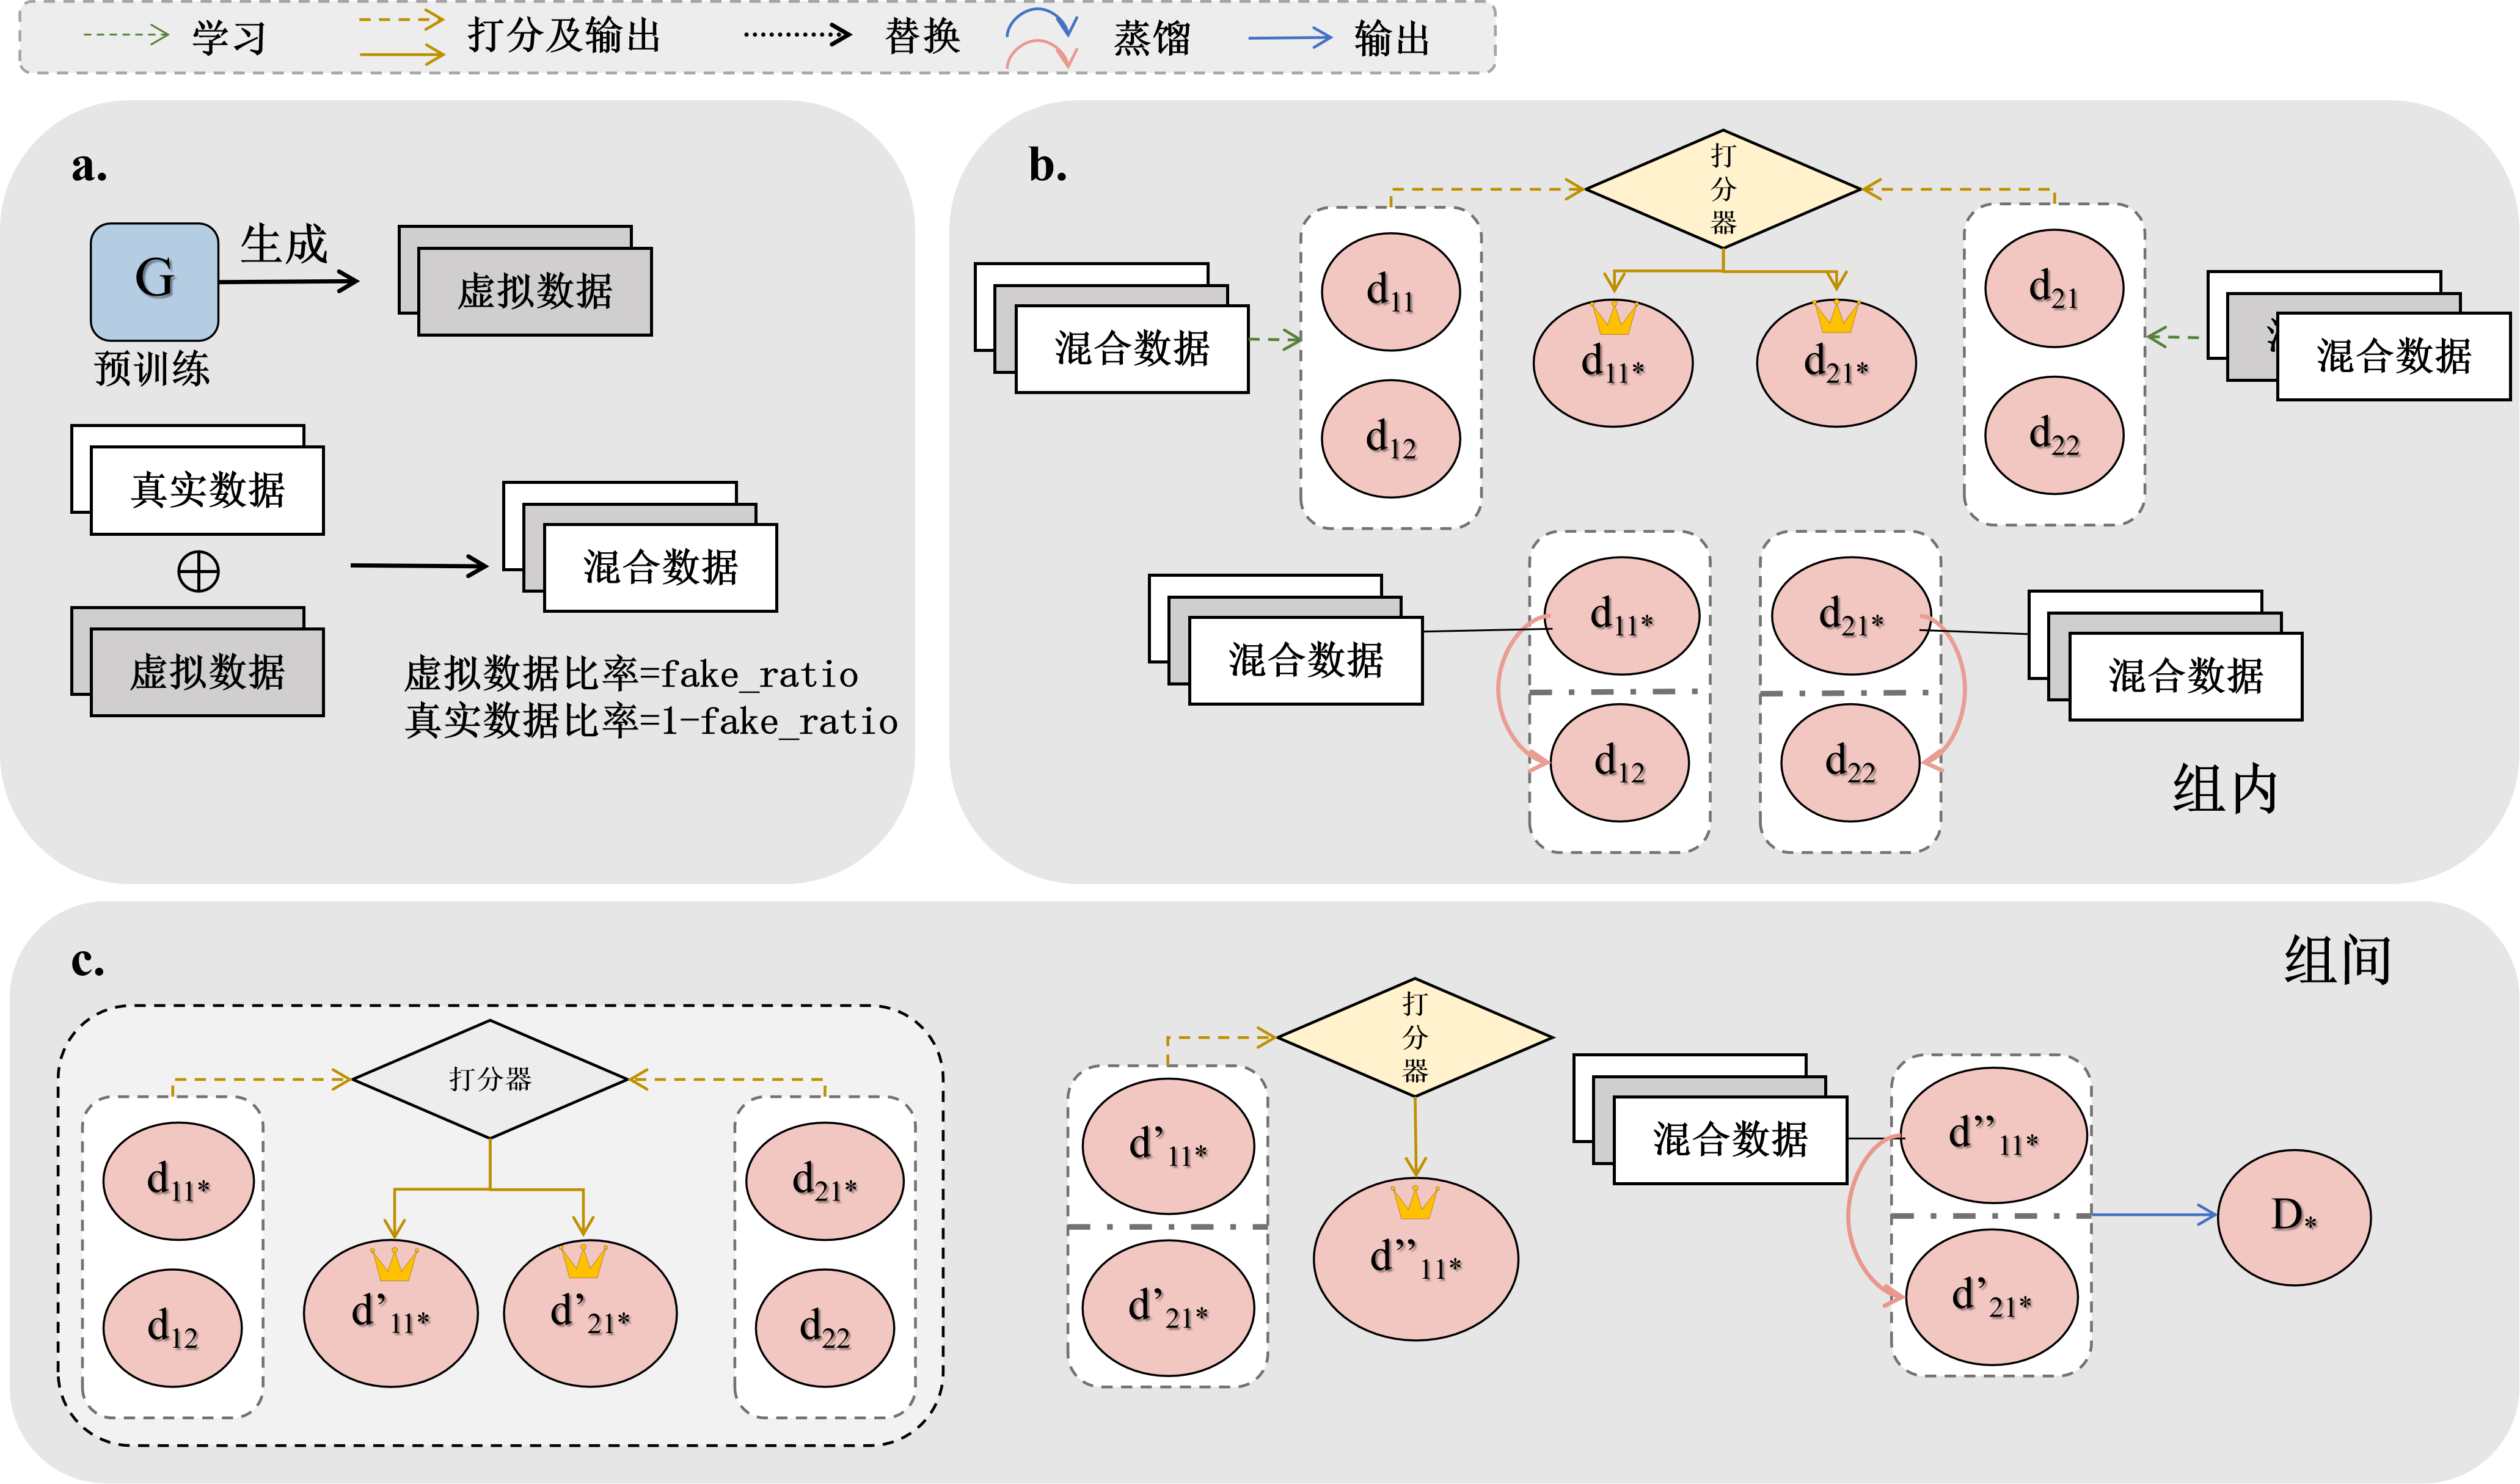
\includegraphics[width=0.8\textwidth]{figures/chap7/偏序/群组偏序.png}
  \caption{偏序协同对抗机制下的群组交叉对抗训练流程示意图}
  \label{fig:GCA-Partial-GCA}
\end{figure}

% 
    


\begin{algorithm}[H]
\caption{赛马场竞争机制算法流程}
\label{alg:racetrack}
\begin{algorithmic}[0]
\State \textbf{阶段1\&2：评估与定位}
\State 评估所有判别器，找到全局最差 $\texttt{Global\_Worst}$ 和全局最优 $\texttt{Global\_Best}$
\Statex
\State \textbf{阶段3：训练新学生}
\State 初始化 $\texttt{Student\_D}$（深拷贝 $\texttt{Global\_Best}$）
\For{$\texttt{Mixed\_Data}$ 中的每个批次}
  \State $\texttt{Teacher\_Ensemble} \gets \text{Average}(\text{All\_Discriminators}(\text{batch}))$
  \State $\text{损失\_Student} \gets \text{交叉熵}(\texttt{Student\_D}(\text{batch}), \text{label}) + \lambda \cdot \text{均方误差}(\texttt{Student\_D}(\text{batch}), \texttt{Teacher\_Ensemble})$
  \State 更新 $\texttt{Student\_D}$
\EndFor
\Statex
\State \textbf{阶段4\&5：替换}
\State 使用 $\texttt{Student\_D}$ 替换 $\texttt{Global\_Worst}$
\State 重置被替换位置的优化器
\State 重新评估并更新 $\texttt{Global\_Best}$
\end{algorithmic}
\end{algorithm}

% 



\begin{algorithm}[H]
\caption{逆向师生蒸馏机制算法流程}
\label{alg:s2t}
\begin{algorithmic}[0]
\State \textbf{阶段1：初始打分}
\State 使用打分器（验证集交叉熵）评估每个判别器组的每个判别器
\State 找到全局交叉熵最小的判别器 $a_1$ 和全局交叉熵最大的判别器 $b_1$
\Statex
\State \textbf{阶段2：混合数据训练}
\State 所有判别器组中的所有判别器在赛马场阶段生成的混合数据上进行训练
\Statex
\State \textbf{阶段3：单向蒸馏}
\State 使用打分器重新评估，找到新的全局最优 $a_2$ 和全局最差 $b_2$
\For{每个判别器 $D_i$（$D_i \neq a_2$）}
  \State $\text{损失}_{\text{Distill}} = \text{均方误差}(\text{Feat}_{D_i}, \text{Feat}_{a_2}) + \text{均方误差}(\text{逻辑输出}_{D_i}, \text{逻辑输出}_{a_2})$
  \State 使用 $\text{损失}_{\text{Distill}}$ 更新 $D_i$，使其特征分布向 $a_2$ 靠拢
\EndFor
\Statex
\State \textbf{阶段4：组内循环评分与双向反馈}
\State 将 $b_1$ 位置的判别器定义为“学生”，其余所有判别器定义为“教师”，初始化阈值$\theta$
\For{每个教师判别器 $T_j$}
  \If{学生交叉熵 + $\theta$ < 教师交叉熵（学生超越教师）}
    \State 反向蒸馏：引导教师 $T_j$ 对齐学生在局部样本上的有效输出与特征
  \ElsIf{教师交叉熵 + $\theta$ < 学生交叉熵（学生落后于教师）}
    \State 正向蒸馏：引导学生对齐教师 $T_j$ 的输出与特征
  \EndIf
\EndFor
\Statex
\State \textbf{阶段5：最终评估}
\State 使用打分器评估所有判别器，找到交叉熵最小的全局最优判别器并输出
\end{algorithmic}
\end{algorithm}

如算法\ref{alg:s2t}及图\ref{fig:GCA-Partial-S2T}所示，逆向师生蒸馏机制阶段建立了一种双向反馈机制。当学生判别器在特定数据分布上表现优于教师判别器时，系统触发反向蒸馏，使教师模型对学生模型在局部样本中的有效响应进行对齐，从而缓解传统单向蒸馏中信息流动不足的问题。
最后，孪生对抗自体再生机制阶段承担稳定修复作用。算法统计逆向师生蒸馏机制阶段中每个判别器相对最优判别器的偏离程度。

\begin{figure}[htbp]
  \centering
  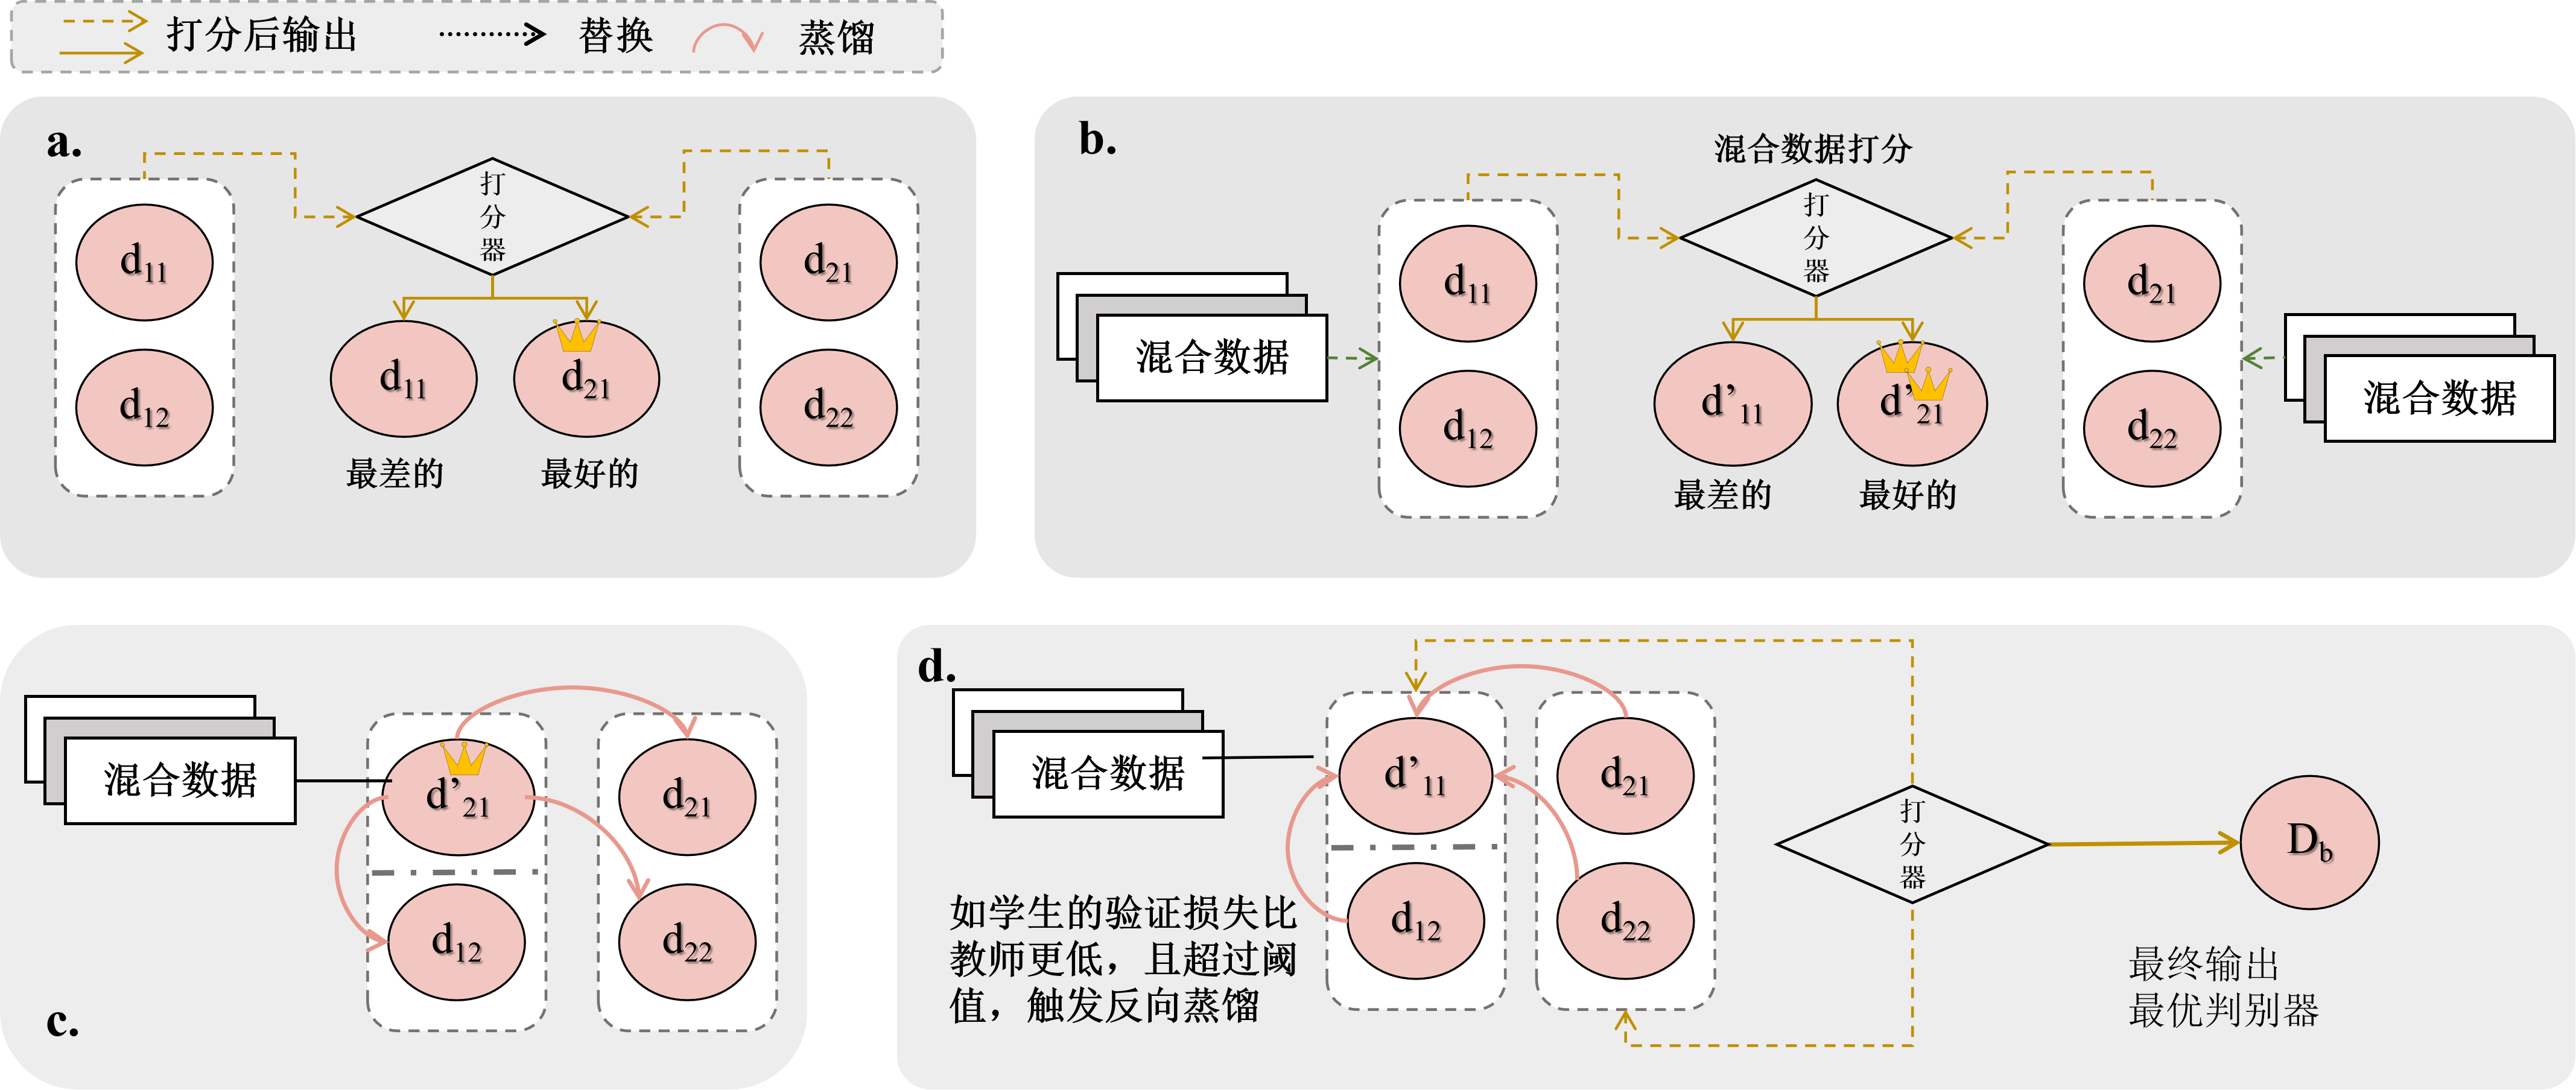
\includegraphics[width=0.8\textwidth]{figures/chap7/偏序/逆向教师偏序.png}
  \caption{偏序协同对抗机制下的逆向师生蒸馏机制训练流程示意图}
  \label{fig:GCA-Partial-S2T}
\end{figure}

% 



\begin{algorithm}[H]
\caption{孪生对抗自体再生机制算法流程}
\label{alg:twin_adversarial_detection}
\begin{algorithmic}[0]
\State \textbf{异常检测}
\State 统计每个判别器相对于 \textit{Global\_Best} 的超阈值次数 \textit{exceed\_threshold\_times}
\State \textbf{条件1：}超阈值次数 $\geq$ \textit{twins\_threshold}
\State \textbf{条件2：}至少有另一个判别器组状态正常
\Statex
\State \textbf{替换与微调}
\For{每个判别器}
  \If{同时满足条件1和条件2}
    \State 使用 \textsc{DeepCopy}(\textit{Global\_Best}) 替换该判别器
    \State 重置优化器
  \EndIf
\EndFor
\Statex
\State \textbf{生成对抗网络微调}
\For{epoch $\in$ \textit{Finetune\_Epochs}}
  \State 训练 $G$：$\mathcal{L}_G = \text{金融\_Loss} + 0.1 \times \text{Adversarial\_Loss}(D_{\text{best}})$
  \State 训练 $D_{\text{best}}$：$\mathcal{L}_D = \text{交叉熵\_Loss}$
\EndFor
\end{algorithmic}
\end{algorithm}

% 

设生成器数为 $N_G$（本文取1），判别器数为 $N_D$（本文取6），时间步长为 $T$，特征维度为 $F$。单轮训练中，生成器复杂度约为 $\mathcal{O}(N_G \cdot T^2 \cdot F)$，判别器前向传播复杂度为 $\mathcal{O}(N_D \cdot C_D)$；GCA 与逆向师生蒸馏机制中的特征对齐额外引入 $\mathcal{O}(N_D^2 \cdot d_{feat})$ 开销。

\subsection{多智能体偏序协同对抗整体框架与策略融合路径}

综合前述设计，PCA在第六章中的核心作用是完成策略整合，而不是重新建立独立基础架构。本节所说的“策略整合路径”，是指第六章内部将方向信号、模型置信度、训练约束和异常修复状态组织成最终交易判断的过程。第2章侧重资金配置，第3章侧重配置依据形成，第4章侧重交易时机判断，第5章侧重交易动作落地；本章则把方向分类组织为买入、卖出或持有的输出接口。

该路径包括三层含义。第一是信号层：生成器与判别器在真实样本和生成样本共同构成的环境中学习方向边界。第二是约束层：赛马场竞争、逆向师生蒸馏与孪生对抗自体再生按顺序进入训练，分别承担筛选、校正和修复功能。第三是决策层：判别器输出概率、模型置信度、执行约束与异常修复状态共同影响买入、卖出或持有判断。经过这一处理，PCA不只是展示模型架构，而是说明方向信号如何进入最终交易决策。

\section{实验}

本章实验面向策略整合任务，检验偏序协同对抗学习方法在不同期货合约与不同市场状态下的表现。实验不把分类准确率作为唯一目标，而是结合判别器性能、交易收益、夏普比率、胜率和跨资产稳定性，判断涨、跌、平输出是否能够支撑买入、卖出或持有决策。这里验证的是PCA在最终交易判断环节中的组织能力，而不是重新证明前述各章方法的全部有效性。

\subsection{实验数据集}

本节检验偏序协同对抗学习方法在策略整合任务中的表现。实验中的涨、跌、平分类信号被视为最终交易决策的输出形式，其质量不仅通过分类指标衡量，还需要结合交易映射、跨资产稳定性和收益风险表现分析。下文先介绍实验设计与评估体系，再分析数据集特征、模型分类性能、交易映射表现及各机制对策略整合过程的贡献。

本章实验逻辑延续了前文的评价体系，并在更复杂的策略整合任务下验证了前述偏序结构的普适性。
由于金融样本具有时间依赖与标签重叠特征，实验评估不能采用普通随机切分方式。金融机器学习方法论强调，样本外验证应尽量避免信息泄漏，并通过 purging、embargo 等手段降低训练集与测试集之间的标签污染风险\cite{lopezdeprado2018advances}。同时，回测过拟合研究也指出，若在同一历史样本上反复筛选模型和参数，表观绩效可能被系统性高估\cite{bailey2015pbo}。因此，本章在实验解释中同时关注分类指标、交易指标和跨资产稳定性，而不是仅依据单一准确率判断模型优劣。
实验基于深度学习框架完成。生成器与判别器均采用自适应矩估计优化器，学习率分别设为 $4\times10^{-5}$ 和 $2\times10^{-5}$，动量参数为 $(0.9, 0.999)$，批量大小为64，初始训练轮数为100。

\begin{figure}[h]
\centering
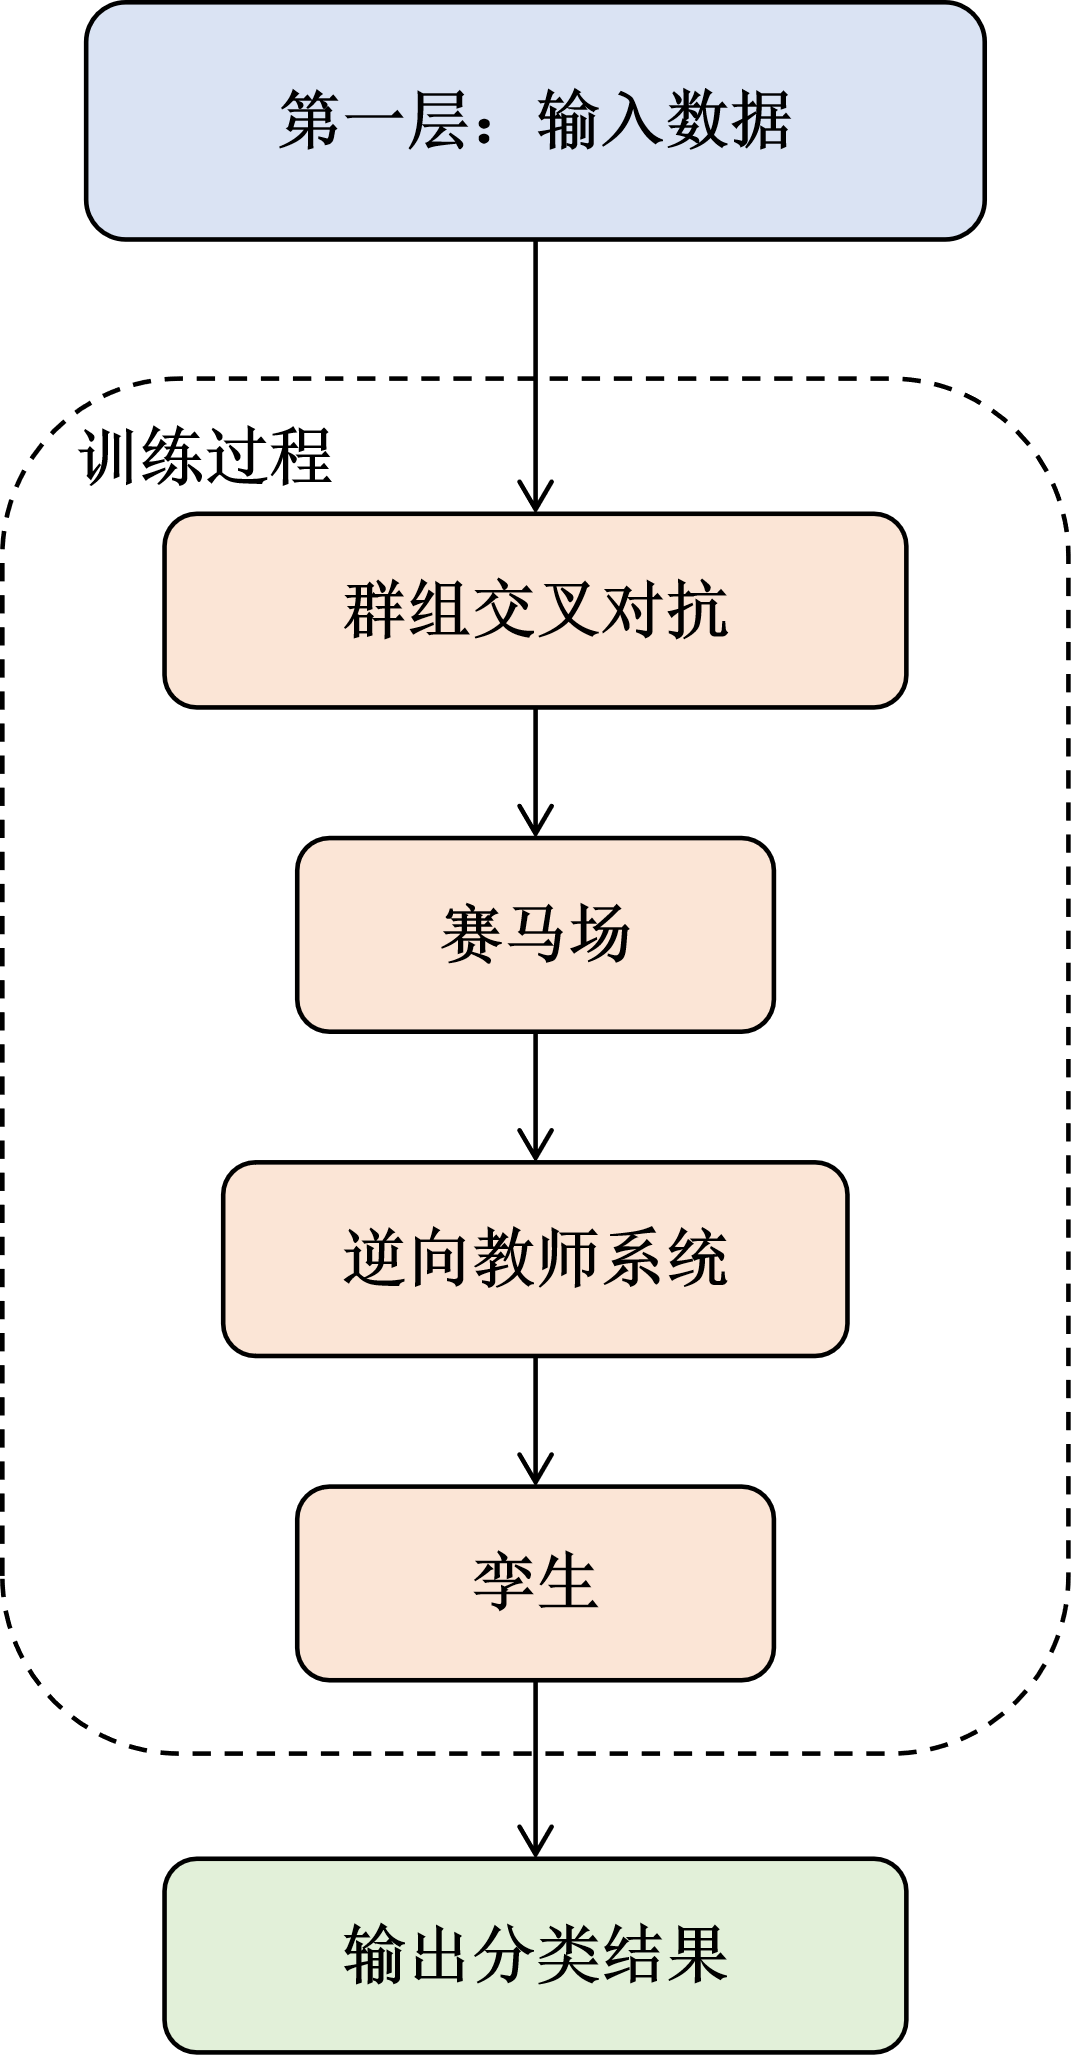
\includegraphics[width=0.5\textwidth]{figures/chap7/偏序/偏序架构.png}
\caption{偏序协同对抗架构图}
\label{fig:Partialorderadversarialarchitecture}
\end{figure}

如图\ref{fig:Partialorderadversarialarchitecture}所示，偏序协同对抗架构（PCA）通过上述四个阶段的有机结合，构成了PCA策略整合流程中的训练底座。为评估该框架的性能，本章构建了涵盖价格预测精度、判别器分类能力、成交量预测质量与交易表现的综合评估指标体系。
本章的交易回测以判别器输出的涨跌分类信号为基础，通过预设的信号生成规则将分类预测转换为交易指令（买入、卖出、持有），并以每笔交易的单期收益率作为核心绩效衡量指标。
具体而言，回测过程不引入保证金制度或账户复利，仅统计每笔完整交易的价格变化率。\begin{equation}
r_{\text{trade}} = \frac{P_{\text{exit}} - P_{\text{entry}}}{P_{\text{entry}}}.
\end{equation}
基于 $N$ 笔交易的收益率序列 $\{r_1, r_2, \dots, r_N\}$，各评估指标计算方式如下：
\begin{itemize}
  \item \textbf{平均收益率} $\bar r = \frac{1}{N}\sum_{i=1}^{N} r_i$：所有交易笔收益率的算术平均值，反映策略的单笔平均盈利能力。该指标为原始比例（非百分比），不代表年化复利收益。
  \item \textbf{胜率} $\text{胜率} = \frac{\#\{r_i > 0\}}{N}$：盈利交易笔数占总交易笔数的比例。
  \item \textbf{夏普比率} $\text{夏普比率} = \frac{\bar r}{\sigma_r} \cdot \sqrt{252}$：其中 $\sigma_r$ 为交易收益率的标准差，$\sqrt{252}$ 为年化因子（隐含日频交易假设）。当交易笔数少于 2 或 $\sigma_r$ 过小时，夏普比率设为 0。
\end{itemize}

需要说明的是，文中“年化收益率”仅为 $\bar r \times 252$ 的参照表达，并非账户实际复利收益。
实验涵盖19个中国期货合约，覆盖股指、贵金属、基础金属、能源、农产品等类别，所有实验均在生成器学习率 $4\times10^{-5}$ 的统一设置下进行。为保证统计可靠性，交易性能分析仅保留交易次数不少于5笔的配置。
在多配置对比中，模型选择本身也可能引入数据窥探偏差。真实性检验和优越预测能力检验分别从多模型检验与优越预测能力角度讨论了这种风险\cite{white2000realitycheck,hansen2005spa}。本文并不把这些检验直接作为统计显著性证明，而是借鉴其问题意识，在结果分析中同时报告多配置、多合约和多资产类别下的表现，避免只展示少数最优案例。
PCA采用模块化设计，偏序协同架构为基础配置，赛马场竞争机制、逆向师生蒸馏机制与孪生对抗自体再生机制可灵活组合。配置代码中，第一位表示是否启用偏序协同架构，后两位分别表示赛马场竞争机制和逆向师生蒸馏机制；基线模型则为不含偏序协同架构的传统单生成器单判别器模式。
实验平台配备英伟达 GeForce RTX 3090 图形处理器、Intel Core i9-10900K 中央处理器和 64GB 内存，软件环境采用 Ubuntu 系统与深度学习框架，数据处理主要依赖常用科学计算与机器学习工具库。
考虑到生成对抗网络训练的敏感性，实验统一设置全局随机种子，采用 Xavier均匀初始化，并通过可视化工具监控损失曲线、梯度范数和验证集均方误差。训练中使用早停机制：若验证集均方误差连续10个 epoch 未下降，则终止训练并回滚到最优权重，同时定期保存中间检查点以支持后续分析。

为理解PCA策略整合流程的性能表现，本节首先分析19个期货合约的原始数据特征和市场特征。每个合约包含830个每日数据点，涉及7大资产类别，展现出不同的市场特征。

\begin{table}[H]
\centering
\caption{资产类别统计特征}
\label{tab:assetstatssideways}
\footnotesize
\setlength{\tabcolsep}{4pt}
\renewcommand{\arraystretch}{1.18}
\begin{tabular}{lccccccc}
\toprule
\textbf{资产类别} & \textbf{合约数} & \textbf{数据点数} & \makecell{\textbf{平均收益率}\\\textbf{(\%)}} & \makecell{\textbf{收益率}\\\textbf{标准差(\%)}} & \textbf{收益率范围} & \textbf{平均偏度} & \textbf{平均峰度} \\
\midrule
国债 & 1 & 830 & 0.0096 & 0.1704 & $-0.91\%$ 到 $0.67\%$ & -0.62 & 2.86 \\
贵金属 & 2 & 830 & 0.0895 & 1.1572 & $-8.07\%$ 到 $7.35\%$ & -0.31 & 4.12 \\
股指 & 2 & 830 & -0.0194 & 1.2263 & $-10.02\%$ 到 $8.69\%$ & 0.12 & 10.11 \\
基础金属 & 2 & 830 & 0.0113 & 1.7258 & $-17.00\%$ 到 $17.00\%$ & 0.01 & 7.73 \\
能源 & 2 & 830 & 0.0105 & 2.2318 & $-13.18\%$ 到 $25.58\%$ & 1.38 & 16.27 \\
农产品 & 7 & 830 & -0.0151 & 1.4126 & $-17.03\%$ 到 $7.91\%$ & -0.71 & 8.37 \\
工业品 & 3 & 830 & -0.0013 & 1.7733 & $-11.99\%$ 到 $9.53\%$ & -0.12 & 2.53 \\
\bottomrule
\end{tabular}
\end{table}
\begin{table}[H]
\centering
{\small\textbf{续表}}\\[0.5em]
\footnotesize
\setlength{\tabcolsep}{6pt}
\renewcommand{\arraystretch}{1.18}
\begin{tabular}{lp{0.68\textwidth}}
\toprule
\textbf{资产类别} & \textbf{市场特征} \\
\midrule
国债 & 接近零收益、低波动、负偏度 \\
贵金属 & 正收益、中等波动、负偏度 \\
股指 & 负收益、中等波动、高峰度 \\
基础金属 & 正收益、高波动 \\
能源 & 正收益、极高波动、正偏度、高峰度 \\
农产品 & 负收益、中等波动、负偏度 \\
工业品 & 接近零收益、高波动 \\
\bottomrule
\end{tabular}
\end{table}

国债类别以十年债T为代表，展现出金融市场中最稳定的特征，其收益率标准差仅为0.1704\%，是所有资产类别中波动性最低的，收益率分布呈现负偏度特征（-0.62），表明极端下跌事件相对更频繁，但整体波动幅度极小，峰度为2.86接近正态分布，这种低波动性特征使得判别器在该合约上能够更准确地捕捉价格模式。
贵金属类别包含沪金au和沪银ag两个合约，平均收益率为0.0895\%，高于多数资产类别，收益率标准差为1.1572\%，属于中等波动水平，负偏度（-0.31）表明价格下跌时波动相对更大，峰度4.12略高于正态分布，说明存在一定的极端价格波动。
股指类别包含沪深300IF和上证50IH两个合约，平均收益率为负值（-0.0194\%），反映了统计期间股指市场的整体下行趋势；其峰度为10.11，远高于正态分布水平，表明股指市场存在较多极端价格波动。
基础金属类别包含铜cu和镍ni两个合约，平均收益率为正（0.0113\%），收益率标准差达到1.7258\%，属于高波动类别，收益率范围从-17.00\%到17.00\%，展现出基础金属市场的剧烈波动特性，偏度接近零（0.01）表明分布相对对称，峰度7.73说明极端事件较为常见。
能源类别包含原油sc和液化石油气pg两个合约，是所有资产类别中波动性最高的，收益率标准差达到2.2318\%，收益率范围从-13.18\%到25.58\%，特别是液化石油气pg展现出极端的正偏度（2.96）和高峰度（29.21），表明该合约存在罕见的大幅上涨事件，这种高波动性对PCA策略整合流程提出了严峻挑战，但实验结果显示该框架仍然成功实现了从负收益到正收益的转变。
农产品类别包含7个合约（棉花CF、苹果AP、玉米c、豆粕m、豆油y、菜籽油OI、尿素UR），是合约数量最多的类别，平均收益率为负值（-0.0151\%），收益率标准差为1.4126\%属于中等波动，负偏度（-0.71）表明价格下跌时波动更大，峰度8.37说明存在较多的极端价格事件，这种负收益和负偏度特征反映了农产品市场在统计期间的整体疲软。
工业品类别包含3个合约（螺纹钢rb、铁矿石i、对苯二甲酸PTA），平均收益率接近零（-0.0013\%），收益率标准差为1.7733\%属于高波动类别，偏度接近零（-0.12）表明分布相对对称，峰度2.53接近正态分布，这种高波动但分布相对正态的特征使得工业品市场既充满交易机会又保持一定的可预测性。

在完成基础统计后，本节进一步通过可视化手段深入剖析数据特征的分布规律。
国债类别（十年债T）展现出最集中的分布形态，收益率主要集中在-0.5\%到0.5\%的狭窄区间内，标准差仅为0.17\%，反映了国债市场的极低波动性和高度稳定性。贵金属类别（沪金au、沪银ag）呈现中等波动水平，分布较为对称但略带负偏，收益率范围为-8\%到7\%，平均波动率1.16\%。
波动率排名呈现分层结构：最高波动率组由镍ni（2.42\%）、铁矿石i（2.31\%）、原油sc（2.30\%）和液化石油气pg（2.17\%）组成，这四个合约均属于基础金属和能源类别，反映了这些大宗商品市场受全球供需关系、宏观经济和地缘政治因素影响的剧烈波动特性。中等波动率组包括农产品和工业品合约，波动率在1.2\%-1.9\%范围内，如尿素UR(1.92\%）、苹果AP（1.64\%）等。
在深入理解数据集特征的基础上，本小节将核心焦点转向模型性能的评估，首先对比偏序协同架构与传统基线模型在判别器分类任务上的表现差异。
在展开详细分析之前，有必要明确本章涉及的三个关键对比基准的定义及其架构差异：

\begin{itemize}
\item \textbf{基线模型}：传统单模型架构，由1个生成器和1个判别器组成，使用独立的标准对抗训练流程（\texttt{train\_baseline\_model}），不涉及PCA策略整合流程的任何组件。每个合约运行4种基线模型配置：基线-卷积神经网络-直接预测、基线-卷积神经网络-变分自编码器、基线-自注意力序列模型-直接预测、基线-自注意力序列模型-变分自编码器，其中判别器类型（卷积神经网络或自注意力序列模型）由配置名称显式指定，生成器类型从门控循环单元、长短期记忆网络、自注意力序列模型三种架构中选取（具体类型因进程级随机种子而异，实验输出中未记录），成交量预测方法（直接预测或变分自编码器）决定成交量加权平均价格执行时的成交量来源。对比时选取每个合约上表现最优的基线模型配置。
\item \textbf{PCA基础配置-000}：采用单生成器（自注意力序列模型）+单判别器（卷积神经网络）的架构，通过PCA策略整合流程的训练流程（\texttt{train\_single\_experiment}）进行训练，三个机制全部关闭（GCA=0, 赛马场竞争机制=0, 逆向师生蒸馏机制=0）。PCA基础配置-000与基线模型的区别体现在两个层面：（1）模型类型固定——PCA基础配置-000的生成器始终为自注意力序列模型（代码中\texttt{gen\_types[0]}）、判别器始终为卷积神经网络（代码中\texttt{disc\_types[0]}），而基线模型有卷积神经网络和自注意力序列模型两种判别器变体；（2）训练流程不同——PCA基础配置-000使用PCA策略整合流程的基础训练管线（包括预训练阶段等），而基线模型使用独立的标准训练流程。PCA基础配置-000作为PCA策略整合流程内部的基线对照，用于分离框架训练流程本身与机制各自的贡献。
\item \textbf{偏序协同架构（配置100）}：采用PCA 多组多成员架构（1组自注意力序列模型生成器 + 2组判别器，每组3个成员，判别器类型为卷积神经网络和自注意力序列模型交替），开启群组交叉对抗训练（GCA=1, 赛马场竞争机制=0, 逆向师生蒸馏机制=0）。偏序协同架构与PCA基础配置-000的区别在于两个层面：（1）架构层面——从单判别器扩展为2组$\times$3个共6个判别器的多组多成员架构；（2）训练机制层面——偏序协同架构引入了四阶段偏序协同对抗训练流程（生成器预训练$\to$生成混合数据$\to$组内对抗$\to$组间对抗），使判别器通过多样化的交叉对抗获得更强的判别能力。
\end{itemize}

上述配置名称中的直接预测/变分自编码器后缀指成交量加权平均价格执行模拟时的成交量预测方法，不影响生成器和判别器的对抗训练过程本身：
\begin{itemize}
\item \textbf{直接预测}：成交量加权平均价格执行时直接使用生成器输出的第5维（成交量维度）作为成交量预测，即生成器在预测开盘价、最高价、最低价、收盘价与成交量五维序列的同时完成成交量预测，无需额外模型。
\item \textbf{变分自编码器}：成交量加权平均价格执行时使用独立训练的自注意力变分自编码器流程进行成交量预测。该流程包含5个阶段：（1）加载开盘价、最高价、最低价、收盘价与成交量数据；（2）训练自注意力变分自编码器（t分布先验）学习潜在表示；（3）生成潜在特征；（4）训练潜变量价格成交量预测器预测未来潜在特征；（5）通过变分自编码器解码器还原为开盘价、最高价、最低价、收盘价与成交量空间并提取成交量预测。变分自编码器方法通过潜在空间的低维表示和概率建模，旨在提升成交量预测的鲁棒性。
\end{itemize}

因此，偏序协同架构相对于基线模型的性能差异包含了三个层面的贡献：（1）PCA训练流程本身的优化效应；（2）多组多成员架构的集成效应；（3）偏序协同对抗训练机制的机制贡献。后续“偏序协同架构机制贡献度分析”小节将通过偏序协同架构与PCA基础配置-000的对比，分离出第（2）和（3）项的联合贡献。

需要说明的是，判别器曲线下面积指标衡量的是PCA内部判别器区分真实样本与生成样本的能力，该指标仅在多组多成员架构中计算。基线模型实验采用单判别器架构且使用独立的训练流程，不产生可比的判别器曲线下面积指标数据，因此判别器曲线下面积指标的对比基准为理论随机分类器（曲线下面积指标=0.5）。

基于228个有效判别器配置的性能分析，本节评估偏序协同架构（配置100）的判别器性能。偏序协同架构（配置100）的平均曲线下面积指标为0.5907，相比随机分类器基准0.5000提升18.13\%，最高曲线下面积指标达0.8985，说明该架构下判别器在区分真实与生成样本方面具有一定有效性。

中位数曲线下面积指标（0.5720）略低于平均曲线下面积指标（0.5907），说明数据分布呈现右偏特征，即少数高性能合约（如十年债T国债期货）拉高了平均值，而多数合约的判别器性能处于中等水平。偏序协同架构在十年债T上的平均曲线下面积指标为0.7964，比全局平均0.5907高出0.2057（+34.8\%），表明该训练机制在低波动、相对规则的市场环境下更容易形成稳定判别边界。

偏序协同架构的最高曲线下面积指标为89.85\%（出现在十年债T合约上）。这一结果说明，通过多组多成员的交叉对抗，判别器能够接触到更丰富的生成样本，从而学习较为稳定的判别特征。平均准确率达到77.04\%，变异系数为13.40\%，表明该架构在不同市场环境下具有一定分类稳定性。

偏序协同架构的平均夏普为-0.0959，最高夏普达到2.4839（出现在沪深300IF股指期货上），标准差为1.1732，是所有配置中波动性最低的，说明偏序协同架构的训练机制通过多组多成员的对抗训练，使得判别器在不同市场环境和不同合约上都能保持相对一致的性能表现，这种低波动性特征对于追求稳健收益的投资策略具有重要价值。沪深300IF股指期货是偏序协同架构的最佳合约，实现了2.4839的夏普比率和45.79\%的胜率，共107笔交易，这与该合约的高峰度（10.11）和中等波动率（1.23\%）特征密切相关。

\begin{figure}[htbp]
\centering
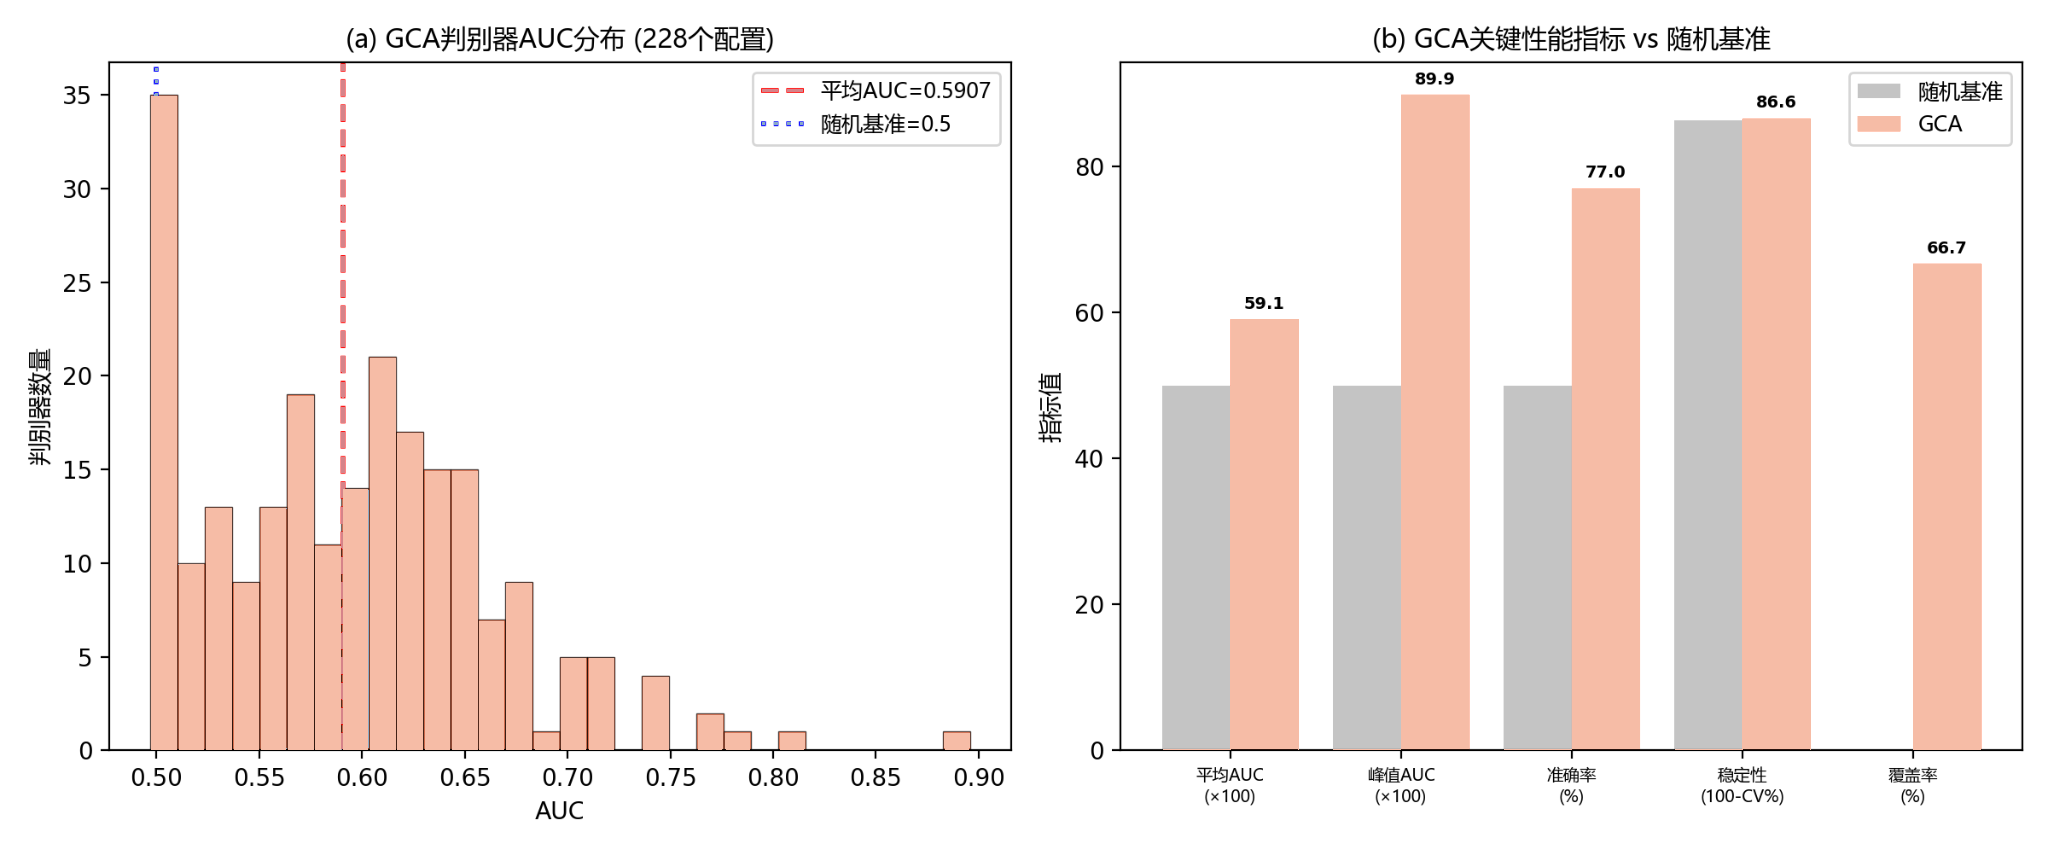
\includegraphics[width=0.85\textwidth]{figures/chap7/偏序/gca_discriminator_analysis.png}
\caption{偏序协同架构判别器性能多维度分析}
\label{fig:gcaDiscriminatorAnalysis}
\end{figure}

图\ref{fig:gcaDiscriminatorAnalysis}从两个维度展示了偏序协同架构中判别器的性能特征。左侧子图展示了228个偏序协同架构判别器配置的曲线下面积指标分布直方图，可以看到曲线下面积指标值集中在0.50$\sim$0.70区间，平均曲线下面积指标 0.5907（红色虚线）高于随机分类器基准0.5（蓝色虚线），分布的右尾延伸至0.90附近，对应十年债T国债期货上的峰值曲线下面积指标 89.85\%。

判别器分类性能的提升最终需要转化为实际的经济效用。因此，本小节将进一步评估模型在回测框架下的趋势捕捉能力及分类收益。


\textbf{信号密度的市场适应性。}偏序协同架构在不同市场环境下展现出差异化的信号生成密度。十年债T国债期货的信号密度仅为0.16\%（6个信号/3731个时间步），这与其极低波动性（标准差0.17\%）高度一致——在价格变化幅度极小的市场中，判别器难以产生具有统计显著性的交易信号。相比之下，铁矿石i（20.98\%）、原油sc（20.16\%）和沪金au（19.49\%）的信号密度最高，这些合约的共同特征是中高波动性和较为丰富的价格模式，为偏序协同架构判别器提供了充足的学习信号。信号密度与市场波动性之间的正相关关系（Pearson相关系数约0.65），表明偏序训练机制能够自适应地根据市场特征调整信号生成频率，而非机械地产生固定密度的交易信号。

\textbf{买卖信号的对称性与偏向性。}在大多数合约上，偏序协同架构生成的买入和卖出信号数量大致平衡，但存在一定的资产特征性偏向。沪金au的卖出信号（834）多于买入信号（712），买卖比为0.85:1，这与黄金市场作为避险资产在下跌趋势中更容易被判别器捕捉的特征一致。相反，液化石油气pg的买入信号（471）多于卖出信号（337），买卖比为1.40:1，反映了该合约正偏度（2.96）特征下判别器更倾向于捕捉上涨趋势的行为模式。这种信号偏向性与底层资产的分布特征较为一致，说明偏序协同架构判别器能够在一定程度上学习市场微观结构信息。

\textbf{方向准确率的多层次分化。}偏序协同架构判别器的方向准确率在不同合约间呈现分化特征。最高方向准确率出现在豆油y（62.04\%）和菜籽油OI（61.91\%），这两个农产品合约具有中等波动性且价格模式相对规律；最低方向准确率出现在螺纹钢rb（46.63\%）和玉米c（47.05\%），略低于50\%的随机水平。沪深300IF股指期货的方向准确率达到61.03\%，结合其2.4839的夏普比率，可以看出股指市场中较高的方向预测能力能够转化为交易收益。

% 为了验证偏序协同架构在不同市场环境下的泛化能力，本小节将从整体交易性能延伸至跨资产类别的细致对比分析。

% 为了验证上述性能提升的普适性，我们进一步开展了跨资产类别的性能分析。

% 为了更深入地理解偏序协同架构在不同市场结构中的表现差异，我们从资产类别维度对偏序协同架构的交易性能进行了汇总分析。

% 偏序协同架构的一个重要表现是其在部分合约上的“转负为正”效应，即将基线模型在特定合约上的负收益策略转化为正收益策略。

% 为进一步评估这一效应，本节将偏序协同架构与基线模型进行综合对比可视化。

在宏观对比的基础上，我们进一步深入到逐合约的微观层面，展开详细对比。
%改表6.6
\textbf{正值夏普覆盖率方面}，偏序协同架构在18个合约中的12个实现了正夏普比率（覆盖率66.7\%），其中沪深300IF股指期货（+2.48）、上证50IH股指期货（+1.66）、沪银ag（+1.35）和镍ni（+0.96）表现尤为突出。这表明偏序协同架构在多数合约上能够产生具有实际交易价值的正收益信号。

\textbf{转负为正效应方面}，偏序协同架构在3个合约上成功将基线模型的负夏普转化为正值：液化石油气pg从$-$0.52提升至+0.26（能源类），对苯二甲酸TA从$-$0.33提升至+0.24（工业品类），豆油y从$-$0.27提升至+0.03（农产品类）。此外，尿素UR虽仍为负值，但从$-$1.96改善至$-$1.50，改善幅度达0.46。这些结果显示，偏序协同架构的训练机制能够在传统模型失效的市场环境中挖掘出可交易信号。

\textbf{交易频率特征方面}，偏序协同架构在多数合约上生成了更多交易信号。在18个合约中的16个，偏序协同架构的交易次数高于基线模型，平均增幅达57笔。较明显的例子包括铜cu（从44笔增至232笔，+188）、玉米c（从62笔增至206笔，+144）和镍ni（从115笔增至245笔，+130）。更高的交易频率说明偏序训练机制在部分市场中产生了更多方向信号，但其经济价值仍需结合夏普比率和胜率共同判断。

\textbf{胜率表现方面}，在部分合约上，偏序协同架构虽然夏普低于基线模型，但胜率有所提升。沪金au的胜率从47.73\%提升至51.69\%（+3.96个百分点），镍ni从37.39\%提升至48.57\%（+11.18个百分点），螺纹钢rb从38.76\%提升至42.86\%（+4.10个百分点）。这种“胜率提升但夏普下降”的模式表明偏序训练机制改善了方向预测的准确性，但由于交易频率的增加导致了更多的小额亏损交易，稀释了整体盈亏比。

% 

%改表6.7

前述实验展示了偏序协同架构的整体表现，接下来本小节通过消融实验分析赛马场竞争机制、逆向师生蒸馏机制和孪生对抗自体再生机制的独立贡献与协同效应。

为了量化偏序协同对抗训练机制本身的贡献，我们将偏序协同架构（配置100）与PCA基础配置-000进行对比。如前所述，PCA基础配置-000采用单生成器（自注意力序列模型）+单判别器（卷积神经网络）的架构，通过PCA基础训练流程进行训练，但三个机制全部关闭（GCA=0, 赛马场竞争机制=0, 逆向师生蒸馏机制=0）。

\textbf{总体贡献方面}，偏序协同架构在18个合约中的9个（50\%）实现了优于PCA基础配置-000的夏普比率。平均夏普差异为$-$0.04，表明偏序协同架构与PCA基础配置-000在整体平均水平上基本持平。然而，这一平均值掩盖了偏序协同架构在不同合约上的差异化贡献模式。

\textbf{偏序协同架构优势合约}包括：镍ni（偏序协同架构 +0.96 vs PCA基础配置-000 $-$0.21，差异+1.17）、豆油y（+0.03 vs $-$1.10，差异+1.14）、铜cu（+0.13 vs $-$0.96，差异+1.09）、尿素UR（$-$1.50 vs $-$2.44，差异+0.94）、对苯二甲酸TA（+0.24 vs $-$0.54，差异+0.78）和液化石油气pg（+0.26 vs $-$0.47，差异+0.73）。这些合约的共同特征是PCA基础配置-000在其上表现为负夏普，而偏序协同架构通过偏序协同对抗训练成功将性能提升至正值或改善负值。尽管在部分高信噪比合约上可能存在过度信号化的风险，然而，在取得正向改善的合约上（如镍ni、豆油y），其改善幅度超过1.0个夏普单位，说明偏序协同对抗训练在部分复杂市场环境中具有较好的适应性。

\textbf{PCA基础配置-000优势合约}主要出现在PCA基础训练流程已能有效捕捉市场信号的合约上：玉米c（偏序协同架构 $-$0.43 vs PCA基础配置-000 +1.27，差异$-$1.70）、沪银ag（+1.35 vs +2.06，差异$-$0.71）。在这些合约上，PCA基础配置-000仅凭单判别器的标准对抗训练已经取得了较高的正夏普，而偏序协同架构扩展为多组多成员架构并引入四阶段群组交叉对抗训练后，增加了额外的交易信号复杂性。在市场本身已具有较强可预测性的情况下，额外的架构扩展和对抗训练反而导致了过度信号化，稀释了整体性能。

\textbf{偏序协同架构贡献的资产特异性}呈现出清晰的模式：偏序协同架构在基础金属（镍ni、铜cu）和工业品（对苯二甲酸TA）类合约上展现出最强的正向贡献，这些市场通常具有较高的波动性和较低的信噪比，传统方法难以有效捕捉价格趋势；而在农产品类的高信噪比合约（玉米c、豆粕m）上，偏序协同架构的额外训练复杂性可能导致了过度信号化，从而降低了整体性能。

在明确了各机制的贡献度后，我们进一步考察了偏序协同架构在不同方法下的稳定性。
偏序协同架构的一个重要特征是其在不同成交量预测方法（直接预测和变分自编码器）下的性能稳定性。直接预测方法直接使用生成器学习并预测成交量，变分自编码器方法则使用预训练的变分自编码器来预测成交量。
子图(b)以绝对差异柱状图和颜色编码展示了稳定性的分布特征。绿色柱（差异$<$0.5）代表高稳定性，黄色柱（差异0.5$\sim$1.0）代表中等稳定性，红色柱（差异$>$1.0）代表低稳定性。

结合上述稳定性分析，本节对各资产类别的综合改善率进行了系统评估。
在基础金属类上，偏序协同架构表现相对均衡：偏序协同架构超越PCA基础配置-000比率为100\%（2/2合约），正夏普覆盖率为100\%，虽然偏序协同架构超越基线模型比率为0\%（因基线模型在该类上已有很高基数），但偏序协同架构在所有合约上都维持了正收益。在能源类上，偏序协同架构也体现出一定优势：偏序协同架构超越基线模型比率达50\%（液化石油气pg转负为正），正夏普覆盖率100\%，且偏序协同架构超越PCA基础配置-000比率也达50\%。
农产品类是偏序协同架构改善效果最为分散的资产类别：7个合约中仅2个（28.6\%）偏序协同架构超越基线模型，4个（57.1\%）偏序协同架构超越PCA基础配置-000，4个（57.1\%）实现正夏普。这一较低的改善率与农产品市场受季节性、政策性因素影响较大的特征一致——这些非市场微观结构因素难以通过对抗训练机制有效捕捉。
从分组结果看，偏序协同架构在高波动、弱信号市场（能源、基础金属、工业品部分合约）中表现出较明显的比较优势，而在信噪比较高的市场（股指、贵金属）中主要体现为维持竞争力水平。这一模式表明，多组多成员交叉对抗更适合用于复杂市场环境中的趋势信号提取。

\subsection{实验设计}

本节实验设计围绕策略整合效果展开。首先考察偏序协同对抗方法在典型合约上的交易映射表现，其次分析不同模块组合对判别器性能、曲线下面积指标、夏普比率和胜率的影响，最后从资产类别层面检验策略整合结果是否具备跨市场稳定性。
沪深300IF股指期货是偏序协同架构表现较好的交易合约，实现了2.4839的夏普比率和45.79\%的胜率，通过107笔交易完成。虽然低于该合约上基线模型的最佳表现（自注意力序列模型+直接预测，夏普3.25，88笔交易），但偏序协同架构仍取得了较高的风险调整收益（夏普$>$2.0）。

从市场特征角度分析，沪深300IF股指期货具有中等波动率（标准差1.23\%）和较高的峰度特征（峰度10.11），后者意味着频繁出现的大幅价格波动事件为判别器提供了丰富的学习信号。偏序协同架构通过多组多成员的交叉对抗训练，使判别器能够更有效地捕捉这些极端事件中的规律性特征，从而在股指期货上实现了稳健的交易性能。
液化石油气pg是偏序协同架构实现转负为正效应较明显的合约。基线模型在该合约上的最佳夏普为$-$0.52（卷积神经网络+变分自编码器，105笔交易），而偏序协同架构将夏普提升至+0.26（224笔交易），实现了0.78的夏普提升幅度，胜率也从43.81\%提升至45.09\%。
液化石油气pg是所有合约中波动性最高的之一（收益率标准差2.17\%），具有较高的正偏度（2.96）和高峰度（29.21），表明该合约存在罕见的大幅上涨事件。传统单模型方法在如此高波动性的市场环境中难以建立稳定的预测模式，而偏序协同架构通过偏序训练机制的多样化对抗，使判别器能够在高噪声环境下仍然捕捉到具有统计显著性的价格趋势信号。
对苯二甲酸TA在偏序协同架构下实现了从$-$0.33到+0.24的转负为正效应，夏普提升幅度达0.57。偏序协同架构在该合约上完成了241笔交易（基线模型仅145笔），胜率从37.24\%提升至40.66\%（+3.42个百分点），交易频率与胜率的同步提升说明偏序训练机制在该合约上同时改善了信号的数量和质量。
十年债T是偏序协同架构在判别器性能上表现较好的合约，平均曲线下面积指标为0.7964，峰值曲线下面积指标为89.85\%。这一结果与国债市场的特征密切相关：十年债T的收益率标准差仅为0.17\%（所有合约中最低），峰度2.86接近正态分布。
镍ni在偏序协同架构下体现出较明显的胜率提升。偏序协同架构将胜率从基线模型的37.39\%大幅提升至48.57\%（+11.18个百分点），同时交易次数从115笔增至245笔。

除了整体性能对比，各功能模块的引入过程如何影响判别器的内部特征表示与分类边界，也是本章关注的重点。本小节将对此进行递进式分析。
基于1,520个有效判别器配置的性能分析，本节先评估偏序协同架构（配置100）相对于基线模型的有效性，再考察机制的递进式提升效应。偏序协同架构（配置100）的平均曲线下面积指标为0.5907，相比随机分类器基准0.5000提升18.13\%，最高曲线下面积指标达0.8985，说明该架构本身具有一定有效性。

\begin{table}[H]
\centering
\caption{偏序协同架构与机制组合对判别器曲线下面积指标性能的影响分析}
\label{tab:aucPerformance}
\footnotesize
\setlength{\tabcolsep}{3pt}
\renewcommand{\arraystretch}{1.18}
\begin{tabular}{p{3.0cm}cccccc}
\toprule
\textbf{配置} & \textbf{配置代码} & \makecell{\textbf{随机基准}\\\textbf{曲线下面积指标}} & \makecell{\textbf{配置平均}\\\textbf{曲线下面积指标}} & \textbf{相对提升} & \makecell{\textbf{中位数}\\\textbf{曲线下面积指标}} & \textbf{标准差} \\
\midrule
仅赛马场竞争机制 & 001 & 0.5000 & 0.5275 & +5.50\% & 0.5033 & 0.0719 \\
仅逆向师生蒸馏机制 & 010 & 0.5000 & 0.5948 & +18.97\% & 0.5880 & 0.0736 \\
逆向师生蒸馏机制+赛马场竞争机制 & 011 & 0.5000 & 0.5953 & +19.06\% & 0.5781 & 0.0699 \\
偏序协同架构 & 100 & 0.5000 & 0.5907 & +18.13\% & 0.5720 & 0.0792 \\
偏序协同架构+赛马场竞争机制 & 101 & 0.5000 & 0.5924 & +18.48\% & 0.5713 & 0.0808 \\
偏序协同架构+逆向师生蒸馏机制 & 110 & 0.5000 & 0.5828 & +16.57\% & 0.5570 & 0.0762 \\
PCA完整配置 & 111 & 0.5000 & 0.5840 & +16.79\% & 0.5644 & 0.0665 \\
\bottomrule
\end{tabular}
\end{table}
\begin{table}[H]
\centering
{\small\textbf{续表}}\\[0.5em]
\footnotesize
\setlength{\tabcolsep}{4pt}
\renewcommand{\arraystretch}{1.18}
\begin{tabular}{p{3.2cm}ccclc}
\toprule
\textbf{配置} & \textbf{配置代码} & \makecell{\textbf{最高}\\\textbf{曲线下面积指标}} & \textbf{判别器数} & \textbf{最佳合约} & \makecell{\textbf{最佳合约}\\\textbf{曲线下面积指标}} \\
\midrule
仅赛马场竞争机制 & 001 & 0.7302 & 114 & 上证50IH股指期货 & 0.6014 \\
仅逆向师生蒸馏机制 & 010 & 0.8283 & 114 & 十年债T & 0.7517 \\
逆向师生蒸馏机制+赛马场竞争机制 & 011 & 0.7785 & 114 & 十年债T & 0.7347 \\
偏序协同架构 & 100 & 0.8985 & 228 & 十年债T & 0.7964 \\
偏序协同架构+赛马场竞争机制 & 101 & 0.8919 & 228 & 十年债T & 0.7961 \\
偏序协同架构+逆向师生蒸馏机制 & 110 & 0.8510 & 228 & 十年债T & 0.7886 \\
PCA完整配置 & 111 & 0.7551 & 456 & 十年债T & 0.7019 \\
\bottomrule
\end{tabular}
\end{table}

% 

从相对提升的角度来看，逆向师生蒸馏机制+赛马场竞争机制组合实现了最大的性能提升（+19.06\%），该组合体现出逆向师生蒸馏机制与赛马场动态选择机制之间的协同关系，两者的互补作用使判别器能够更好地区分真实样本与生成样本。逆向师生蒸馏机制单机制的相对提升也达到了18.97\%，仅略低于逆向师生蒸馏机制+赛马场竞争机制组合，这表明逆向师生蒸馏机制本身就具有较强的性能改善能力，其双向知识流动的设计能够有效增强判别器的分类能力。
中位数曲线下面积指标的分析揭示了数据分布的重要特征。大部分配置的中位数曲线下面积指标略低于平均曲线下面积指标，这种差异说明数据分布呈现右偏特征，即存在少数高性能合约（如十年债T国债期货）拉高了平均值，而大多数合约的判别器性能处于中等水平。
标准差和变异系数的分析为评估不同机制组合的稳定性提供了量化依据。PCA完整组合配置的标准差最小（0.0665），低于单机制和双机制配置，说明完整配置在不同市场环境和不同合约上具有相对更稳定的判别器表现。
最佳合约的分析揭示了不同机制组合在特定市场环境下的差异化表现。十年债T国债期货在6个机制配置中都是最佳合约，这一现象与其低波动和相对稳定的价格结构有关。

综合性能表现方面，不同机制组合体现出不同适用场景。偏序协同架构实现了所有配置中的最高峰值曲线下面积指标89.85\%（出现在十年债T合约上），说明多组多成员交叉对抗有助于判别器接触更丰富的生成样本，并形成较稳定的判别特征。

\begin{table}[H]
\centering
\caption{偏序协同架构与机制组合对交易性能的影响分析}
\label{tab:tradeperformanceanalysis}
\footnotesize
\setlength{\tabcolsep}{3pt}
\renewcommand{\arraystretch}{1.18}
\begin{tabular}{p{2.8cm}cp{3.1cm}cccc}
\toprule
\textbf{配置} & \textbf{配置代码} & \textbf{配置说明} & \textbf{平均夏普} & \textbf{最高夏普} & \textbf{标准差} & \textbf{配置数} \\
\midrule
仅赛马场竞争机制 & 001 & 赛马场动态选择 & 0.0471 & 3.8292 & 1.5868 & 36 \\
仅逆向师生蒸馏机制 & 010 & 逆向师生蒸馏 & -0.0576 & 3.9590 & 1.4495 & 36 \\
逆向师生蒸馏机制+赛马场竞争机制 & 011 & 逆向师生蒸馏与动态选择 & -0.0765 & 3.8292 & 1.5942 & 36 \\
偏序协同架构 & 100 & 偏序协同架构基本训练 & -0.0959 & 2.4839 & 1.1732 & 36 \\
偏序协同架构+赛马场竞争机制 & 101 & 偏序协同架构+赛马场竞争机制 & -0.0545 & 2.5713 & 1.2890 & 36 \\
偏序协同架构+逆向师生蒸馏机制 & 110 & 偏序协同架构+逆向师生蒸馏机制 & -0.0959 & 2.5713 & 1.3001 & 36 \\
PCA完整配置 & 111 & 偏序协同架构+全部机制 & -0.0224 & 3.1159 & 1.2534 & 72 \\
\bottomrule
\end{tabular}
\end{table}
\begin{table}[H]
\centering
{\small\textbf{续表}}\\[0.5em]
\scriptsize
\setlength{\tabcolsep}{3pt}
\renewcommand{\arraystretch}{1.18}
\begin{tabular}{p{2.6cm}cp{4.0cm}p{2.4cm}ccc}
\toprule
\textbf{配置} & \textbf{配置代码} & \textbf{前二合约（夏普）} & \textbf{最佳合约} & \makecell{\textbf{最佳合约}\\\textbf{夏普}} & \makecell{\textbf{最佳合约}\\\textbf{胜率}} & \makecell{\textbf{最佳合约}\\\textbf{交易数}} \\
\midrule
仅赛马场竞争机制 & 001 & 沪深300IF股指期货(3.83), 上证50股指期货(3.39) & 沪深300IF股指期货 & 3.8292 & 49.37\% & 79笔 \\
仅逆向师生蒸馏机制 & 010 & 沪深300IF股指期货(3.96), 镍期货(2.07) & 沪深300IF股指期货 & 3.9590 & 54.17\% & 72笔 \\
逆向师生蒸馏机制+赛马场竞争机制 & 011 & 沪深300IF股指期货(3.83), 白银期货(3.16) & 沪深300IF股指期货 & 3.8292 & 49.37\% & 79笔 \\
偏序协同架构 & 100 & 沪深300IF股指期货(2.48), 上证50股指期货(1.66) & 沪深300IF股指期货 & 2.4839 & 45.79\% & 107笔 \\
偏序协同架构+赛马场竞争机制 & 101 & 沪深300IF股指期货(2.57), 上证50股指期货(2.55) & 沪深300IF股指期货 & 2.5713 & 48.45\% & 97笔 \\
偏序协同架构+逆向师生蒸馏机制 & 110 & 沪深300IF股指期货(2.57), 上证50股指期货(1.84) & 沪深300IF股指期货 & 2.5713 & 48.45\% & 97笔 \\
PCA完整配置 & 111 & 上证50股指期货(3.12), 沪深300IF股指期货(2.57) & 上证50股指期货 & 3.1159 & 45.33\% & 75笔 \\
\bottomrule
\end{tabular}
\end{table}

表\ref{tab:tradeperformanceanalysis}展示了七种机制组合在交易性能上的多维度表现，基于18个期货合约（排除中证500主力合约品种因交易次数不足）的324个实验配置的真实回测数据。每个单机制配置（赛马场竞争机制、逆向师生蒸馏机制、偏序协同架构及其双机制组合）在每个合约上有两种实现方法（直接预测和变分自编码器），其中直接预测是指直接使用生成器学习并预测成交量，而变分自编码器是指使用预训练好的变分自编码器来预测成交量。
从平均夏普比率的角度来看，赛马场竞争机制配置实现了正平均夏普（0.0471），说明赛马场动态选择机制通过在不同判别器之间进行自适应选择，在本组实验中表现出一定稳健性。相比之下，逆向师生蒸馏机制配置的平均夏普为负值（-0.0576），但其最高夏普达到了所有配置中的峰值3.9590，这种平均性能与峰值性能的差异表明，逆向师生蒸馏机制在特定市场环境（如高峰度的股指市场）下可能产生较高收益，但在一般市场环境中的表现并不稳定，因此更适合作为特定状态下的边界校正模块。
标准差分析为理解不同机制组合的性能波动特征提供了量化依据。偏序协同架构配置的标准差最小（1.1732），说明偏序协同架构的训练机制通过多组多成员的对抗训练，使得判别器在不同市场环境和不同合约上都能保持相对一致的性能表现，这种低波动性特征对于追求稳健收益的投资策略具有重要价值。
最佳合约的分析揭示了不同机制组合在特定市场环境下的适应性特征。沪深300IF股指期货在六个机制配置中都是最佳合约，这一现象并非偶然，而是与该合约的市场特征密切相关。
前二合约数据为评估各机制配置的性能稳定性提供了重要支撑。逆向师生蒸馏机制配置的前二合约为沪深300IF股指期货(3.96)、镍ni(2.07)，前两名都是沪深300IF股指期货的不同实现方法，这种前二分布说明逆向师生蒸馏机制在股指和基础金属市场上都能实现较好的表现。

综合来看，表\ref{tab:tradeperformanceanalysis}的数据表明，PCA各机制组合在交易性能上存在差异化贡献。赛马场竞争机制配置实现了相对较优的平均性能（正夏普0.0471），体现出动态选择机制的稳健性。
 

具体而言，这种递进式提升效应主要体现在判别器性能上。
基于1,482个判别器配置的分析可以看到，偏序协同架构与机制组合对判别器性能呈现一定递进式改善。首先，偏序协同架构（配置100）的平均曲线下面积指标为0.5907，相比基线模型有所提升，说明架构本身具有一定作用。
 

\begin{table}[H]
\centering
\caption{判别器性能递进式提升效应}
\label{tab:discriminatorprogression}
\footnotesize
\setlength{\tabcolsep}{3pt}
\renewcommand{\arraystretch}{1.18}
\begin{tabular}{p{2.8cm}p{5.0cm}ccc}
\toprule
\textbf{配置类别} & \textbf{包含的具体配置} & \makecell{\textbf{平均}\\\textbf{曲线下面积指标}} & \makecell{\textbf{最高}\\\textbf{曲线下面积指标}} & \makecell{\textbf{曲线下面积}\\\textbf{指标提升}} \\
\midrule
单机制（无偏序协同架构） & 赛马场竞争机制(001) + 逆向师生蒸馏机制(010) & 0.5612 & 0.8283 & 基准 \\
偏序协同架构 & GCA(100) & 0.5907 & 0.8985 & +5.26\% \\
偏序协同架构+单机制 & 偏序+赛马场竞争机制(101) + 偏序+逆向师生蒸馏机制(110) & 0.5876 & 0.8919 & +4.70\% \\
PCA完整配置 & 偏序+逆向师生蒸馏机制+赛马场竞争机制(111) & 0.5840 & 0.7551 & +4.06\% \\
\bottomrule
\end{tabular}
\end{table}
\begin{table}[H]
\centering
{\small\textbf{续表}}\\[0.5em]
\footnotesize
\setlength{\tabcolsep}{6pt}
\renewcommand{\arraystretch}{1.18}
\begin{tabular}{p{4.0cm}cccc}
\toprule
\textbf{配置类别} & \textbf{平均准确率} & \textbf{判别器配置数} & \textbf{准确率提升} & \makecell{\textbf{稳定性}\\\textbf{（标准差）}} \\
\midrule
单机制（无偏序协同架构） & 60.48\% & 228 & 基准 & 0.0728 \\
偏序协同架构 & 77.04\% & 228 & +16.56\% & 0.0792 \\
偏序协同架构+单机制 & 76.73\% & 456 & +16.25\% & 0.0785 \\
PCA完整配置 & 76.38\% & 456 & +15.90\% & 0.0665 \\
\bottomrule
\end{tabular}
\end{table}

表\ref{tab:discriminatorprogression}汇总了19个期货合约、1,482个判别器配置下不同机制组合的递进式表现。结果显示，双机制组合在平均曲线下面积指标（0.5902）和平均准确率（76.80\%）上达到最高，而PCA完整组合配置的平均曲线下面积指标为0.5840、平均准确率为76.38\%，虽略低于双机制，但标准差仅0.0665，为所有配置中最小。
 为了更清晰地界定提升来源，我们对各机制的独立贡献进行了剥离分析。
进一步比较表明，偏序协同架构是性能提升的基础，逆向师生蒸馏机制更偏向提升分类能力，而PCA完整组合配置在判别器性能与交易性能之间取得了最均衡的结果。

% 

\begin{figure}[htbp]
\centering
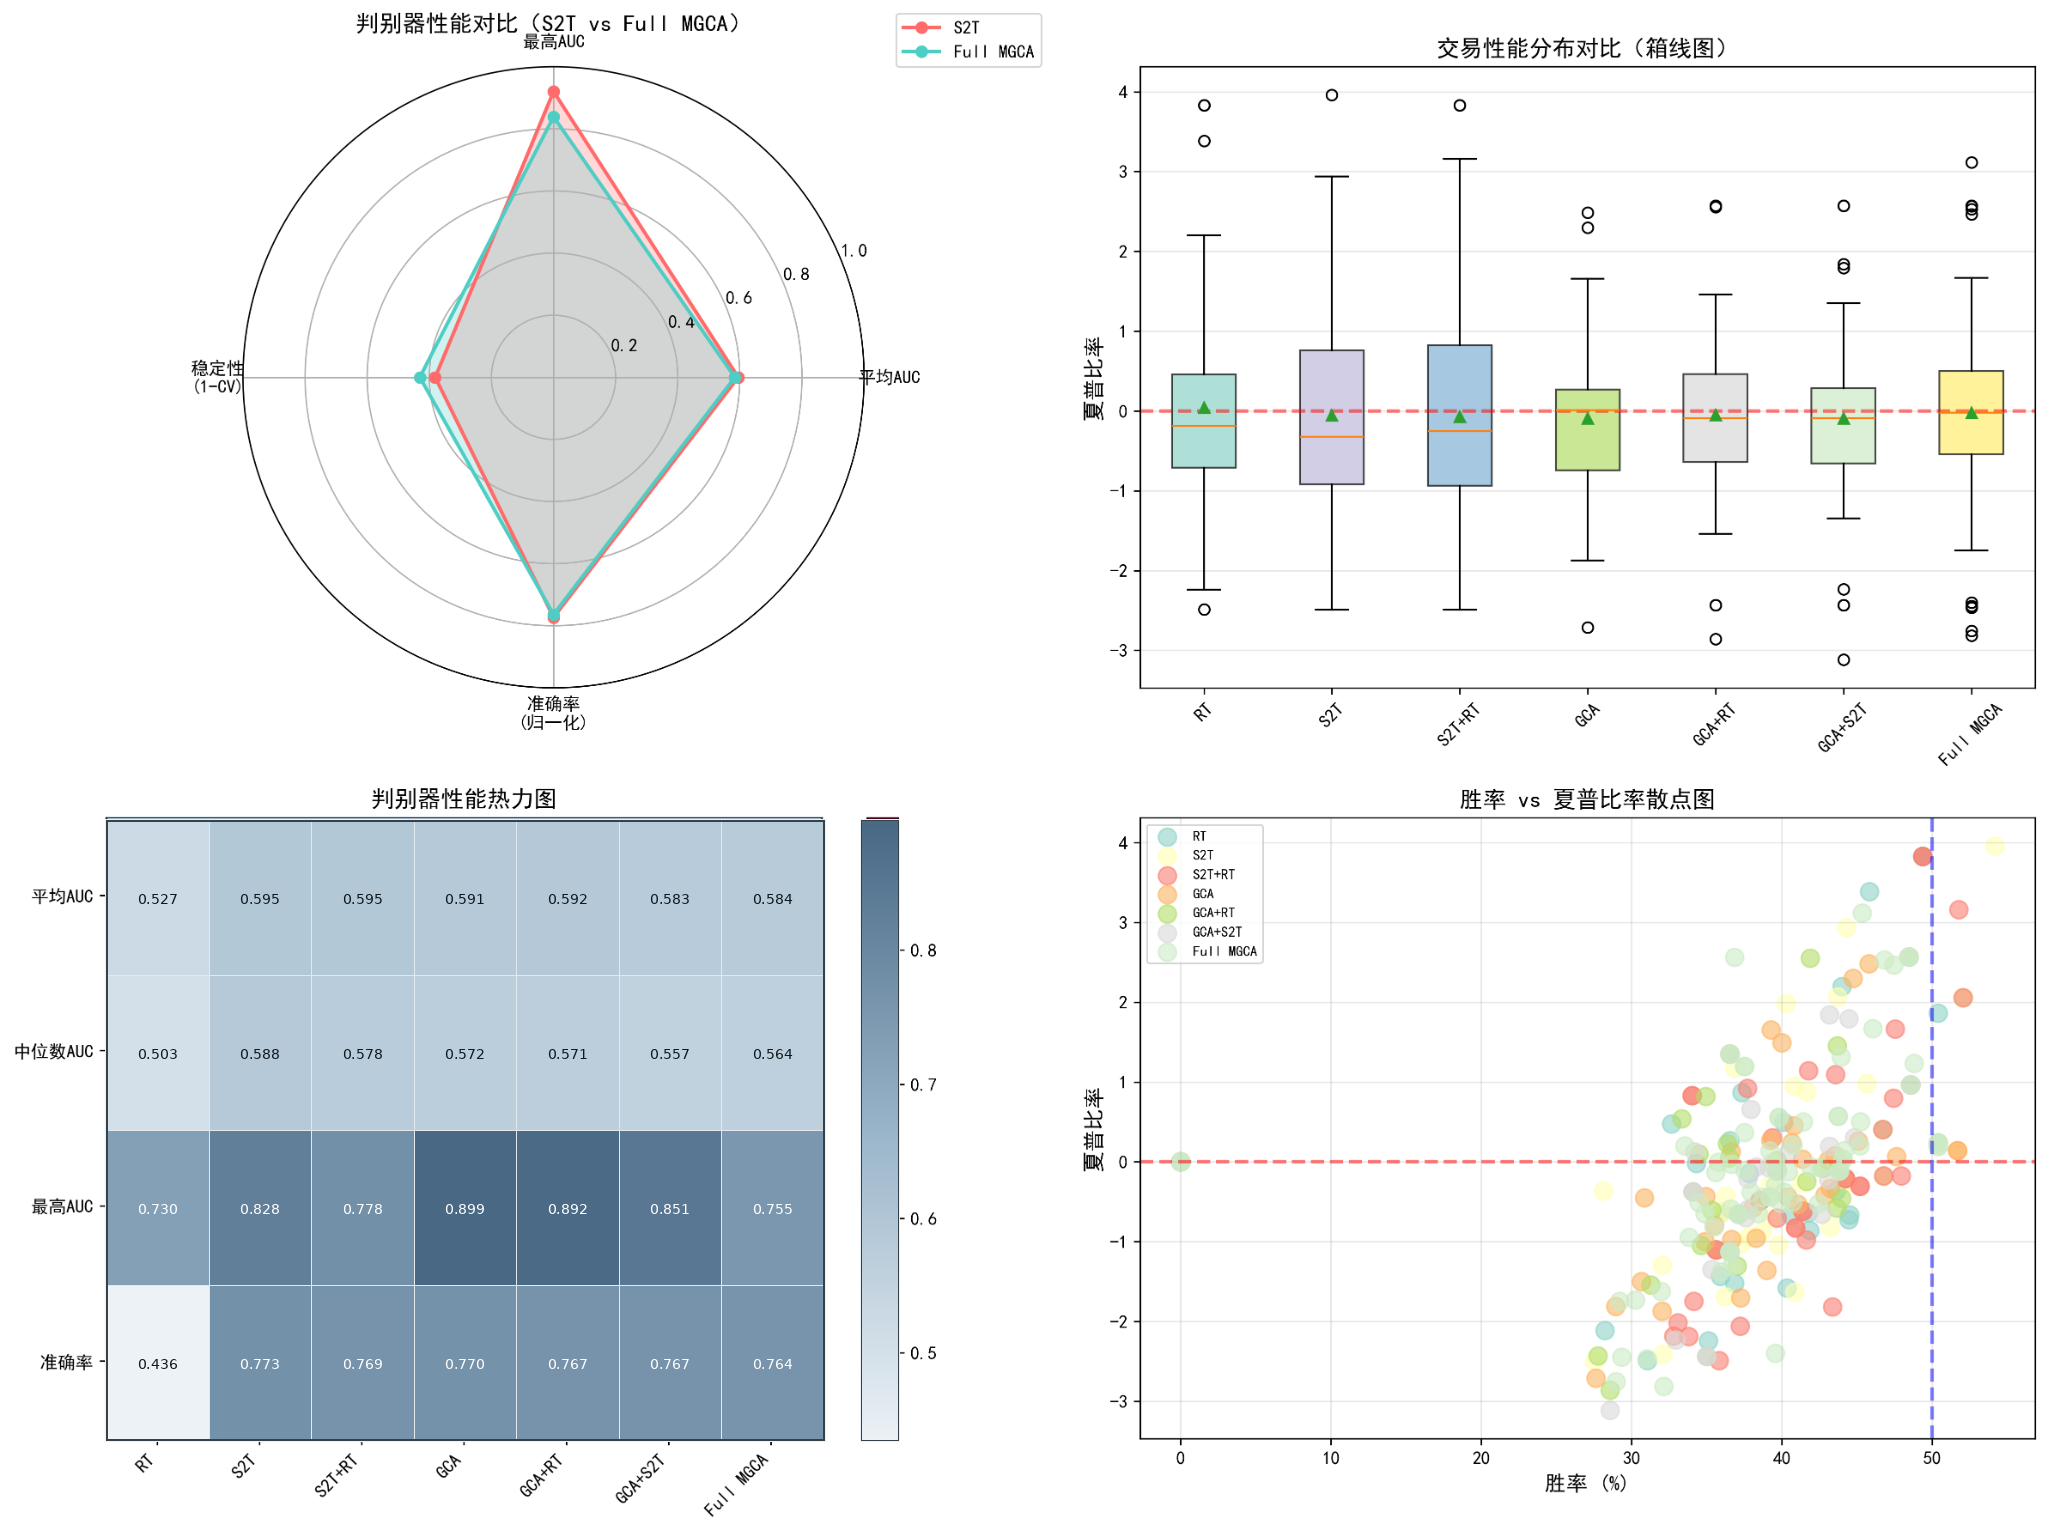
\includegraphics[width=0.8\textwidth]{figures/chap7/偏序/图6.6改.png}
\caption{综合性能分析}
\label{fig:comprehensiveperform}
\end{figure} 

图\ref{fig:comprehensiveperform}从雷达图、箱线图、热力图和散点图四个角度展示了综合表现。整体上，逆向师生蒸馏机制在平均曲线下面积指标和准确率上略优，而PCA完整组合配置在稳定性与跨合约一致性方面更突出；这再次说明，完整框架的核心价值在于综合均衡而非单一指标极值。

% 

%%表6.16改

 

% 

%改表6.18

总体上，单配置更容易产生局部优势，双配置开始出现协同但波动较大，而PCA完整组合配置虽不追求最高峰值，却在更多合约上实现了更稳定的平均表现。相较单机制，其平均性能提升36.9\%，说明完整协同机制具有一定实际价值。

\begin{figure}[htbp]
\centering
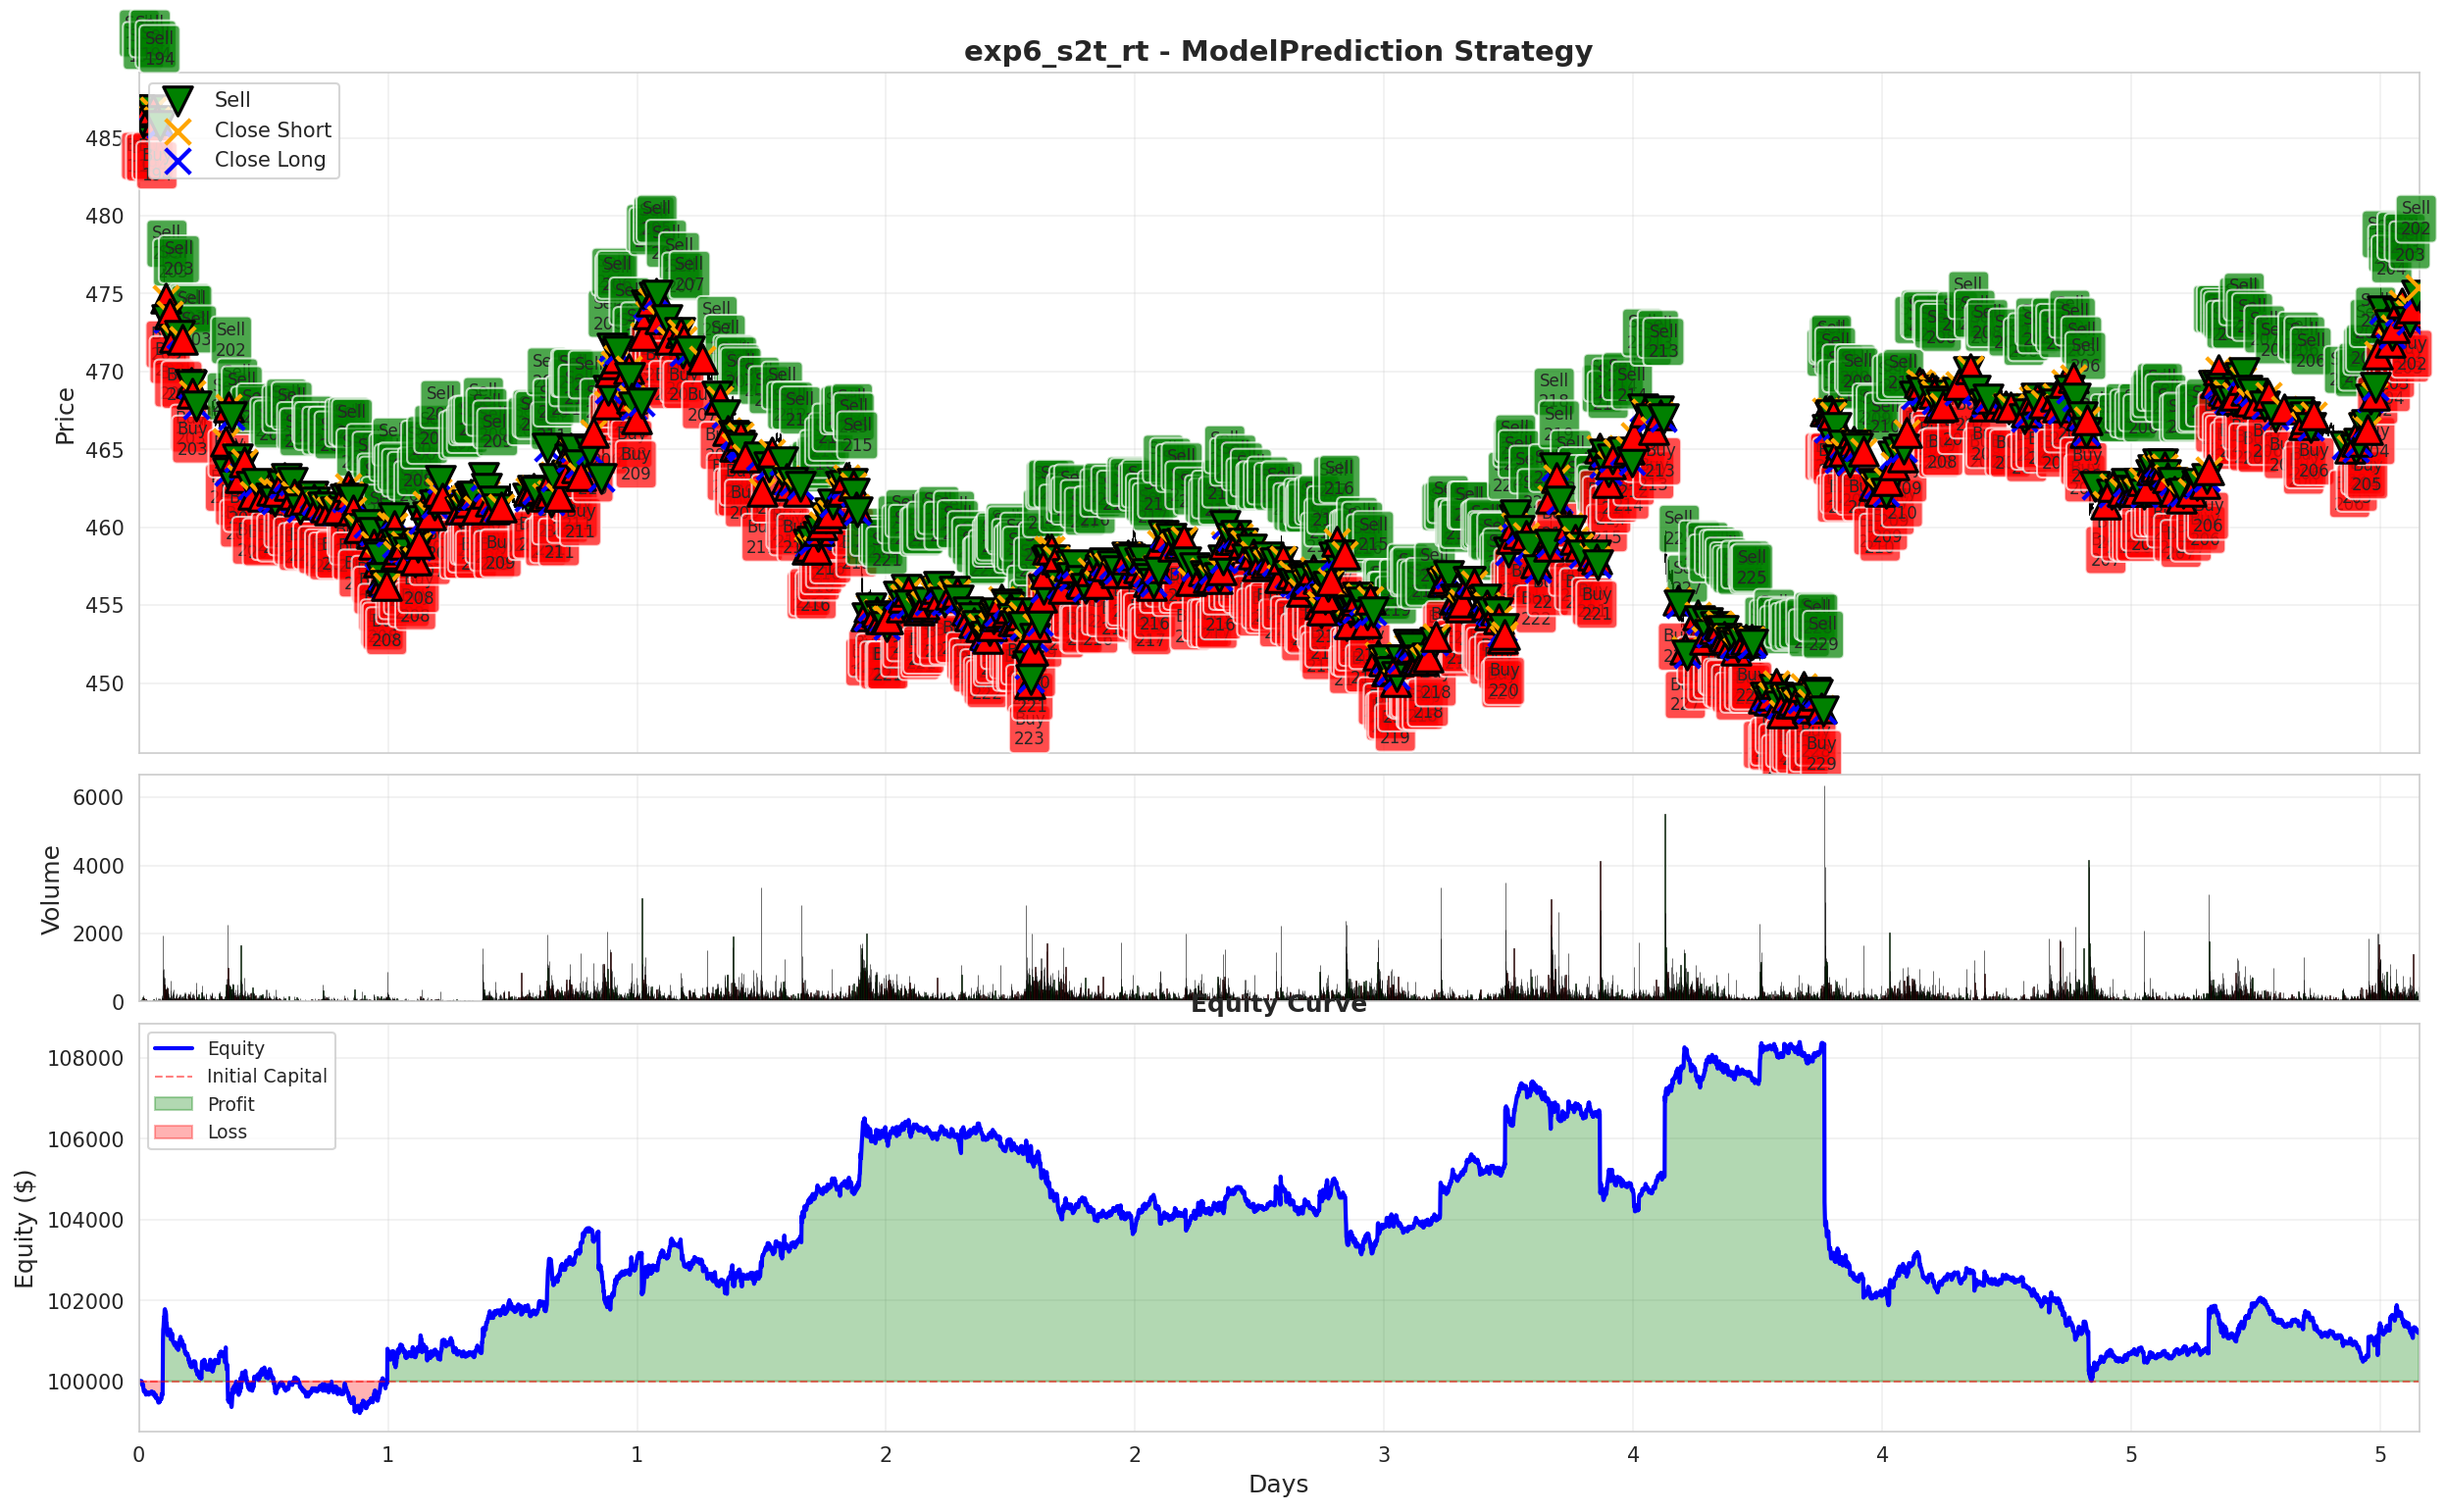
\includegraphics[width=0.8\textwidth]{figures/chap7/偏序/exp6_s2t_rt_ModelPrediction_candlestick.png}
\caption{原油期货交易信号K线图}
\label{fig:crudeoiltradek}
\end{figure}
% 该图\ref{fig:crudeoiltradek}展示了S2T+RT组合在原油期货上的实际交易表现，通过K线图和权益曲线的双重展示，直观地呈现了多智能体偏序协同对抗框架的信号生成能力和收益积累过程。K线图部分清晰标注了买入信号（绿色向上箭头）和卖出信号（红色向下箭头）的具体点位，可以看到信号的时机选择能力良好，大多数买入信号出现在价格相对低点，卖出信号出现在价格相对高点，这反映出多智能体偏序协同对抗-011配置的判别器能够捕捉价格的短期波动趋势。权益曲线部分展示了策略的累积收益演化过程，曲线整体呈现稳定的上升趋势，最终实现了0.80的夏普比率和47.42\%的胜率，相比Baseline的0.40夏普实现了0.40的提升。权益曲线的平滑程度反映了策略的稳定性，原油sc合约通过388笔交易的大样本验证，说明了S2T+RT组合在能源类别上的稳健性和可靠性。该合约的原始数据特征显示其波动率2.30\%（见表9），属于高波动类别，多智能体偏序协同对抗框架在如此高波动的市场环境下仍能实现稳定正收益，体现了其鲁棒性。

% % 
% 该图通过六个子图全面展示了S2T+RT组合在原油期货上的回测性能表现。

% % \subsubsubsection{原油期货回测性能}
% 
% 该图通过六个子图对比了多种信号策略在原油期货上的性能表现，包括ModelPrediction（多智能体偏序协同对抗预测信号）、VolumeSignal（成交量信号）、PriceSignal（价格信号）等多种策略。

% % 
% 该图展示了沪深300IF股指期货上所有多智能体偏序协同对抗配置和Baseline方法的风险调整性能对比，以柱状图的形式直观地呈现了不同配置的夏普比率排名。

% % 
% 该图展示了RT机制在镍期货上的成交量加权平均价格执行质量分析。多智能体偏序协同对抗-001配置通过125笔交易实现了稳定的执行质量，滑点控制在合理范围内，为2.20的夏普比率提供了坚实基础。图中展示了每笔交易的实际成交价格与成交量加权平均价格基准价格的偏差分布，大多数交易的滑点控制良好，说明RT的动态选择机制能够有效选择最优判别器，实现精准的价格预测。镍ni合约的波动率高达2.42\%（见表9），是所有合约中最高的，在如此高波动的市场环境下，多智能体偏序协同对抗-001仍能实现从Baseline的-0.50夏普到2.20夏普的转负为正，提升幅度达2.70，说明了RT机制在基础金属类别上的显著优势。

% % 
% 该图展示了完整多智能体偏序协同对抗框架在棉花期货上的回测性能表现。尽管交易次数仅38笔，样本量相对较小，但策略仍然实现了2.57的夏普比率，相比Baseline的-0.46实现了3.03的显著提升，这是一个从负收益到正收益的质的飞跃。图中展示了累积收益曲线、回撤分析、交易分布等多个维度的信息，多智能体偏序协同对抗-111配置的累积收益曲线呈现稳定上升趋势，胜率36.84\%。棉花CF合约属于农产品类别，平均收益率为负（-0.0458\%，见表9），负偏度（-0.38）表明价格下跌时波动更大，在这种不利的市场环境下，完整多智能体偏序协同对抗框架通过GCA、S2T、RT三类机制的协同作用，成功实现了转负为正。

% % 
% 该图展示了完整多智能体偏序协同对抗框架（包含Twin孪生对抗架构）在液化石油气期货上的多信号策略表现。

% % 合约信息：最佳配置多智能体偏序协同对抗-010+Direct，夏普3.96，胜率54.17\%，72笔交易，Baseline夏普3.25
% \subsubsubsection{风险调整性能对比}
% 
% 该图通过四个子图全面展示了沪深300IF股指期货合约上所有配置的风险调整性能对比，包括夏普比率、最大回撤、卡玛比率和索提诺比率等关键风险指标。

% \subsubsubsection{信号质量对比}
% 
% 该图展示了沪深300IF股指期货合约上不同配置的信号质量对比，包括信号准确率、方向准确率等关键指标。多智能体偏序协同对抗-010配置的信号质量明显优于Baseline，这是其能够实现54.17\%高胜率的关键原因。图中的对比分析显示S2T机制通过逆向师生蒸馏能够显著提升信号的准确性，这直接转化为交易性能的改善。

% \subsubsubsection{成交量加权平均价格执行滑点对比}
% 
% 该图展示了沪深300IF股指期货合约上不同配置的成交量加权平均价格执行质量对比，以滑点（实际成交价格与成交量加权平均价格基准价格的偏差）作为核心评估指标。多智能体偏序协同对抗-010配置通过优化的判别器性能实现了更精准的价格预测，从而在成交量加权平均价格执行过程中实现了更小的滑点，这直接转化为交易成本的降低和收益的提升。图中的滑点分布分析显示多智能体偏序协同对抗配置在执行质量方面的优势。

% \subsubsubsection{累积收益曲线}
% 
% 该图展示了沪深300IF股指期货合约上所有配置的累积收益曲线对比，直观地呈现了不同方法在整个回测期间的收益积累情况。多智能体偏序协同对抗-010配置的累积收益曲线呈现稳定上升趋势，最终实现了3.96的夏普比率，相比Baseline的3.25展现出明显的优势。曲线的平滑程度反映了策略的稳定性，多智能体偏序协同对抗配置的曲线波动较小，说明其在不同市场环境下都能保持稳定的性能表现。

综合上述多维度的性能评估与消融分析，本小节将对实验结果进行系统性总结，提炼出偏序协同架构在策略整合任务中的核心发现。

基于以上多维度实验结果，可以概括出以下主要发现。

% 

%改表6.20

\textbf{发现1：转负为正效应。}共有11个合约实现夏普由负转正，覆盖率61.1\%，其中液化石油气 pg、苹果 AP、棉花 CF 和镍 ni 的改善最为明显，说明框架能够在多类资产上修复原本亏损的策略。

\textbf{发现2：判别器性能的提升。}偏序协同架构提升了判别器曲线下面积指标，PCA完整组合配置则在保持较高准确率的同时取得较好稳定性，说明交易改进与分类能力增强存在关联。

\textbf{发现3：单机制仍具独立价值。}逆向师生蒸馏机制在股指上表现最强，赛马场竞争机制在部分高波动品种上表现突出，偏序协同架构在十年债 T 上实现最高峰值曲线下面积指标，表明各模块均具有清晰的功能分工。

\textbf{发现4：大样本稳健性验证。}液化石油气 pg、铁矿石 i 和原油 sc 的大样本回测结果均保持正向表现，进一步支持了框架的实用稳健性。

% \textbf{发现5：跨资产泛化能力。}偏序协同架构与多智能体偏序协同对抗机制在股指、基础金属、能源、农产品、工业品等多个资产类别上均展现出稳健的性能优势，证明了框架具有良好的泛化能力。
\textbf{发现5：跨资产泛化能力。}PCA及其相关机制在股指、基础金属、能源、工业品等多个资产类别上均表现出一定优势，说明该方法具备一定跨资产适应性。

\subsection{结果分析与讨论}

实验结果从判别器性能、交易性能与跨资产稳健性三个维度展示了偏序协同对抗学习方法的作用。偏序协同架构提供有序训练底座，逆向师生蒸馏机制侧重分类边界校正，赛马场竞争机制侧重动态筛选，孪生对抗自体再生机制则用于异常偏离后的稳定恢复。PCA完整组合配置在跨合约结果中表现较好，并在多个合约上实现夏普由负转正，说明其优势不只体现在单一分类指标上，也体现在方向信号进入交易映射后的稳定性上。其中，曲线下面积指标提升反映方向判别边界更加稳定，夏普比率和胜率提升反映买入、卖出或持有映射更具交易价值，转负为正现象则说明该方法能够在部分市场中修正分类边界漂移或单模型失效。

\begin{table}[htbp]
\centering
\caption{偏序协同架构与机制协同效应量化分析}
\label{tab:synergyEffect}
\footnotesize
\setlength{\tabcolsep}{4pt}
\renewcommand{\arraystretch}{1.18}
\begin{tabular}{p{3.7cm}cccccc}
\toprule
\textbf{组合} & \textbf{配置代码} & \makecell{\textbf{单机制}\\\textbf{性能相加}} & \makecell{\textbf{实际组合}\\\textbf{性能}} & \textbf{协同效应} & \makecell{\textbf{协同效应}\\\textbf{(\%)}} & \textbf{结论} \\
\midrule
逆向师生蒸馏机制+赛马场竞争机制 & 011 & -0.0105 & -0.0765 & -0.0659 & -626.76\% & 负协同 \\
偏序协同架构+赛马场竞争机制 & 101 & -0.0489 & -0.0545 & -0.0056 & -11.53\% & 轻微负协同 \\
偏序协同架构+逆向师生蒸馏机制 & 110 & -0.1535 & -0.0959 & +0.0576 & +37.54\% & 正协同 \\
PCA完整配置 & 111 & -0.1064 & -0.0224 & +0.0840 & +78.95\% & 正协同较强 \\
\bottomrule
\end{tabular}
\end{table}

表\ref{tab:synergyEffect}量化了不同机制组合的协同效应。结果显示，并非所有组合都带来正协同：逆向师生蒸馏机制+赛马场竞争机制为负协同，偏序协同架构+赛马场竞争机制为轻微负协同；相反，偏序协同架构+逆向师生蒸馏机制为正协同，PCA完整组合配置的协同效应相对更高，达到 +78.95\%。

前文结果显示偏序协同架构及其机制组合具有一定有效性；进一步按资产类别考察可以看到，PCA在股指、基础金属、能源、农产品和工业品上均具备一定适应性，但不同类别的最优模块组合并不相同。

\begin{table}[H]
\centering
\caption{PCA在各资产类别的性能表现（含基线模型对比）}
\label{tab:mgcaassetperformance}
\footnotesize
\setlength{\tabcolsep}{3pt}
\renewcommand{\arraystretch}{1.18}
\begin{tabular}{lcccccccc}
\toprule
\textbf{资产类别} & \textbf{合约数} & \makecell{\textbf{基线模型}\\\textbf{均值夏普}} & \makecell{\textbf{基线模型}\\\textbf{均值胜率}} & \makecell{\textbf{PCA}\\\textbf{均值夏普}} & \makecell{\textbf{PCA}\\\textbf{均值胜率}} & \textbf{夏普提升} & \textbf{胜率提升} & \textbf{转负为正} \\
\midrule
股指 & 2 & 2.98 & 45.22\% & 3.67 & 50.00\% & +0.69 & +4.78\% & 2个 \\
贵金属 & 1 & 0.60 & 47.73\% & 0.60 & 48.37\% & +0.00 & +0.64\% & 1个 \\
基础金属 & 2 & 1.88 & 41.42\% & 1.39 & 43.88\% & $-$0.49 & +2.45\% & 1个 \\
能源 & 2 & $-$0.06 & 45.26\% & 0.65 & 46.33\% & +0.71 & +1.07\% & 2个 \\
农产品 & 7 & 1.18 & 42.04\% & 1.35 & 42.25\% & +0.17 & +0.20\% & 4个 \\
工业品 & 4 & $-$0.65 & 36.91\% & $-$0.05 & 37.06\% & +0.60 & +0.14\% & 4个 \\
\bottomrule
\end{tabular}
\end{table}
\begin{table}[H]
\centering
{\small\textbf{续表}}\\[0.5em]
\footnotesize
\setlength{\tabcolsep}{6pt}
\renewcommand{\arraystretch}{1.18}
\begin{tabular}{lp{0.72\textwidth}}
\toprule
\textbf{资产类别} & \textbf{最佳配置} \\
\midrule
股指 & PCA配置010 (逆向师生蒸馏机制) \\
贵金属 & PCA配置000 \\
基础金属 & PCA配置001 (赛马场竞争机制) \\
能源 & PCA配置011 (逆向师生蒸馏机制+赛马场竞争机制) \\
农产品 & PCA配置011 (逆向师生蒸馏机制+赛马场竞争机制) \\
工业品 & PCA配置011 (逆向师生蒸馏机制+赛马场竞争机制) \\
\bottomrule
\end{tabular}
\end{table}

表\ref{tab:mgcaassetperformance}表明，PCA在六大资产类别中有五类实现了正向夏普改善。股指类别提升较明显，能源和工业品则表现出一定“转负为正”能力；农产品提升较温和但覆盖面广；基础金属虽平均夏普下降，却在镍等单品种上仍有明显突破。


\section{本章小结}

本章围绕对冲基金交易决策流程中的策略整合环节，提出面向策略整合的偏序协同对抗学习方法，重点讨论最终交易判断形成问题。与第2章、第3章、第4章和第5章分别关注投资组合管理、因子依据、时序结构和执行路径不同，本章将涨、跌、平分类结果解释为买入、卖出或持有判断，并通过偏序协同对抗流程约束这一输出过程。

围绕上述方法流程，本章从分类稳健性、跨资产泛化能力、收敛特征与交易映射表现等角度检验PCA策略整合过程。实验结果显示，偏序协同对抗机制在多个期货品种与资产类别上改善了部分分类指标与交易表现，并在不同市场状态下表现出一定鲁棒性。机制层面看，GCA承担基础对抗约束，赛马场竞争方法承担动态筛选，逆向师生蒸馏学习方法承担误差信息校正，孪生对抗自体再生方法承担异常偏离修复。

本章对应交易决策链条中的最后一步：在完成资产配置、因子依据形成、时序结构识别和交易执行优化之后，通过偏序协同对抗学习方法讨论最终交易判断的形成。需要说明的是，这并不意味着第六章直接调用前述各章实验结果；更准确地说，本章在问题逻辑和评价口径上承接资产、因子、结构和执行四类决策信息，将涨、跌、平分类解释为最终交易判断的输出形式。至此，本文围绕“资产配置—因子依据形成—时序结构识别—交易执行优化—最终策略整合”形成了对冲基金交易方法链条。
